% !TeX root = ../main.tex

\chapter{Resultados e Discussões \label{chap:resultados}}


Com o método de otimização proposto realizamos experimentos de classificação e recuperação de formas pelo conteúdo, para dois descritores, com a base de folhas de plantas Flavia \cite{4458016},  que possui $1907$ imagens de folhas de $32$ espécies. A Figura \ref{fig:bases} ilustra imagens das folhas desta base. Cada exemplar ilustrado foi segmentado e colorido de acordo com a espécie ao qual pertence. Essa base de folhas é amplamente utilizada na validação de trabalhos de reconhecimento automático de espécies de plantas. 

\begin{figure}[!htb]
\caption{\label{fig:bases}Amostras de formas de folhas da base de imagens Flavia.}

\centering
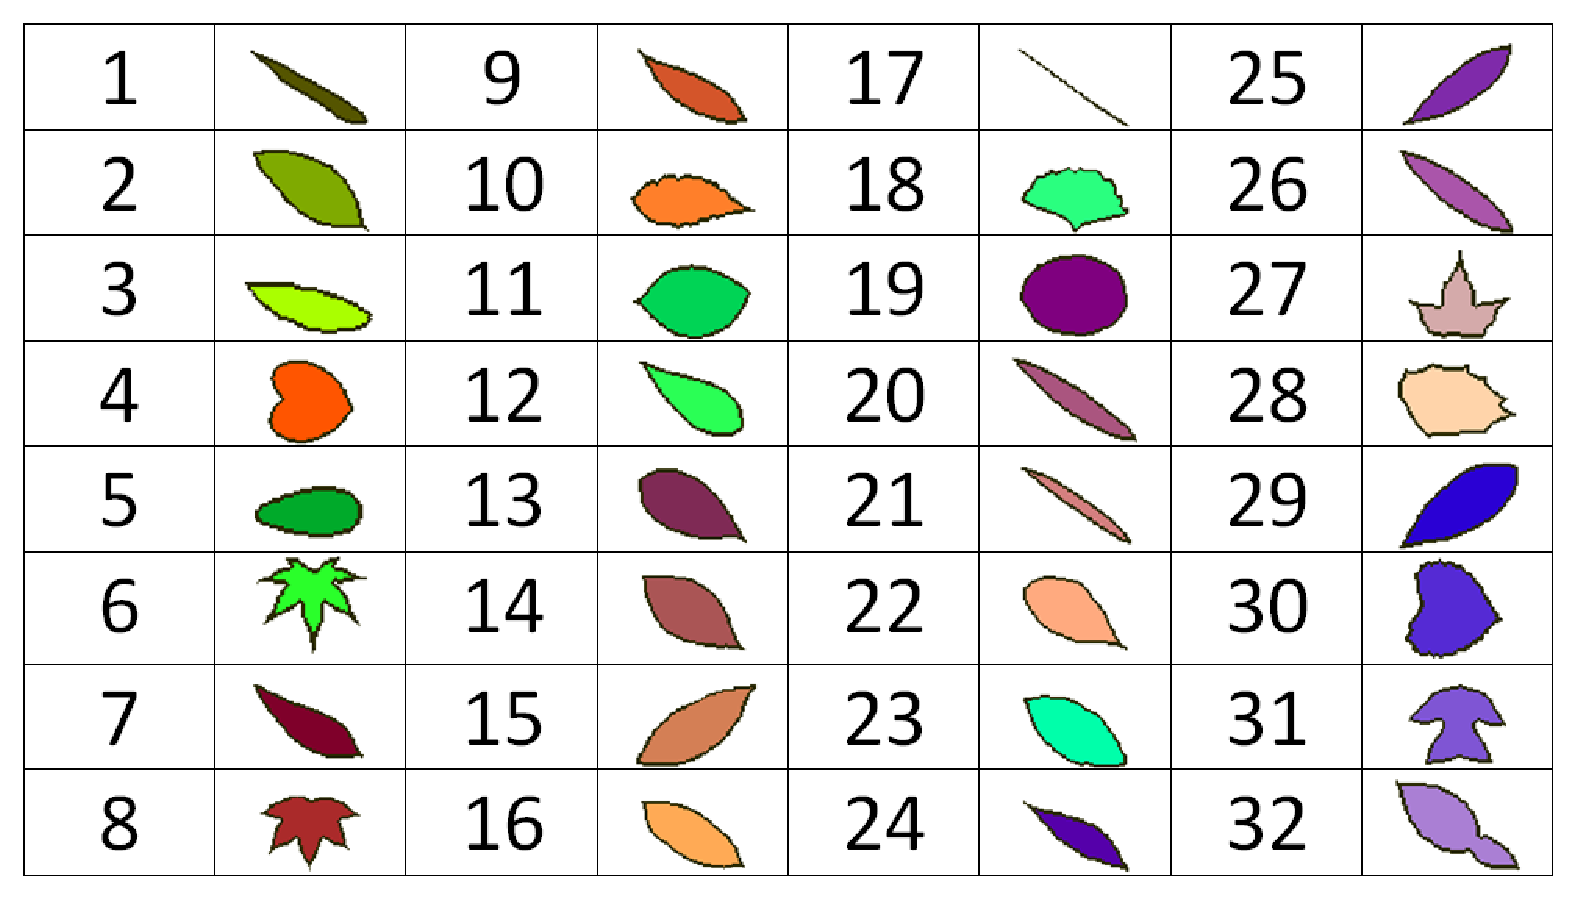
\includegraphics[width=0.5\textwidth]{fig5.eps}
\end{figure}




\section{\emph{Classificação de formas e sua relação com  a função objetivo}}
Nos experimentos realizados para comparação dos algoritmos de otimização avaliamos inicialmente aspectos  relacionados à  convergência dos algoritmos de otimização e a relação entre os resultados de classificação e as funções MADs obtidas por diferentes estratégias. Além disso investigamos o custo computacional dos mesmos. A Figura \ref{fig:converge} ilustra a convergência de cada um dos três algoritmos de otimização para $30$ repetições realizadas em um subconjunto da base de formas de folhas de plantas. Os resultados obtidos indicam que a otimização realizada pelo \emph{PSO} requereu um pequeno número de iterações para convergir para uma solução ótima, quando comparado aos algoritmos \emph{SA} e \emph{DE}. Uma vez que a convergência está relacionada com o número de iterações necessárias para se atingir uma solução ótima, um menor número de iterações implica em em exploração deficiente do espaço de busca, ou seja, em convergência prematura \citeonline{Andries:2007}. Nestes casos, o método de otimização apresenta tendência de ficar preso a mínimos locais, encontrando assim soluções sub-ótimas para o problema. Por outro lado, a convergência mais lenta permite ao algoritmo explorar melhor o espaço de busca, aumentando portanto a chance deste convergir para um mínimo global, ou seja, uma solução ótima \citeonline{Andries:2007}.
 
Neste contexto, observa-se na Figura \ref{fig:converge}c que o \emph{PSO} encontrou soluções sub-ótimas com maior frequência, alcançando valores médios da função MAD  igual a $0,805 \pm 0,006$.  Com relação aos algoritmos \emph{SA} e \emph{DE}, estes alcançaram os menores valores médios de MAD : $0,795 \pm 0,006$ e $0,798 \pm 0,004$, respectivamente. Esses resultados demonstram que os algoritmos \emph{SA} e \emph{DE} foram mais eficazes que o \emph{PSO} em encontrar soluções ótimas. No entanto, o custo para alcançar tais soluções torna-se maior. A Seção \ref{sec:comp_cost} aborda com mais detalhes as questões relativas ao custo computacional dos algoritmos de otimização utilizados.

\begin{figure}[!htb]
\caption{\label{fig:converge} Convergência dos métodos de otimização para o problema de descrição de folhas de plantas: (a) SA, (b) DE, (c) PSO. As curvas em vermelho destacam o valor médio da função MAD para $30$ realizações de cada método (curvas em preto).} 

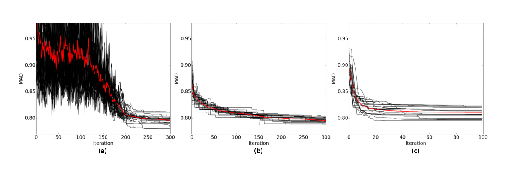
\includegraphics[width = \textwidth]{fig6.eps}
\end{figure}

A análise corrente tem como hipótese o fato de que as escalas otimizadas e o valor ótimo de MAD, que estão inter-relacionadas, implicam em melhorias na taxa de acerto da classificação das espécies vegetais. A Tabela \ref{tab:leaves_supervised_results} exibe os diversos valores de MAD e os correspondentes resultados obtidos nos experimentos de classificação para diferentes classificadores. Observa-se que os melhores resultados de classificação correspondem aos menores valores de MAD obtidos através da metodologia de otimização de parâmetros. Os resultados de classificação para o descritor \emph{NMBE}, com as escalas ajustadas conforme sugerido por \citeonline{Costa:1997} ($\operatorname{NMBE_{orig}}$), resultou em um desempenho intermediário quando comparado aos resultados para escalas otimizadas e escolhidas arbitrariamente. Os resultados mostram que o descritor \emph{NMBE} otimizado ($\operatorname{NMBE_{opt}}$) melhorou o desempenho de todos os classificadores avaliados, uma vez que este alcançou as maiores taxas de Precisão e Revocação para os menores valores de MAD, o que confirma a hipótese inicial.

Apesar do descritor \emph{NMBE} ter sido originalmente projetado para descrição de formas de neurônios, nesta tese o aplicamos com sucesso em caracterização de folhas de plantas, uma vez que a metodologia de otimização o ajustou ao problema em questão.
É importante ressaltar que os diferentes algoritmos de otimização, atingiram valores de MAD distintos, e portanto conjuntos de escalas otimizadas distintos, os resultados de classificação corroboraram a hipótese e a conclusão anterior, pois tais conjuntos de escalas  permitiram com que os descritores fossem capazes de capturar detalhes dos contornos das formas e as diferenciasse apropriadamente. Com isso observamos que os algoritmos de otimização trazem vantagens à representação multiescala com impacto significativo na caracterização das folhas. 

\begin{table}[]
\begin{minipage}{\textwidth}
\renewcommand\footnoterule{}
\caption{Valores de MAD e resultados de classificação das espécies vegetais da base de imagens Flavia para diferentes estratégias de escolha das escalas do descritor \emph{NMBE}. }
\label{tab:leaves_supervised_results}
\resizebox{\textwidth}{!}{ 
\begin{tabular}{cccccccccc}
\toprule[1.5pt]
 & \multicolumn{8}{c}{Classifier} \\ \cmidrule(lr){2-9} 
 & \multicolumn{2}{c}{NB}  & \multicolumn{2}{c}{Knn (n = 5)}  & \multicolumn{2}{c}{LDA}  & \multicolumn{2}{c}{QDA} \\
\cmidrule(lr){2-3}  \cmidrule(lr){4-5} \cmidrule(lr){6-7}  \cmidrule(lr){8-9}
MAD & Precision & Recall & Precision & Recall & Precision & Recall & Precision & Recall \\ \midrule
$0,762$\footnote{Using SA}        & ${0,91 \pm 0,02}$   & ${0,89 \pm 0,02}$         & ${0,93 \pm 0,02}$          & ${0,92 \pm 0,02}$         & ${0,87  \pm 0,02}$          & ${0,85\pm 0,02}$         & ${0,95  \pm 0,01}$          & ${0,94  \pm 0,01}$         \\
$0,783$\footnote{Using DE}        & $0,88 \pm 0,02$          & $0,87\pm0,02$         & $0,90\pm0,02$          & $0,88\pm0,02$         & $0,85\pm0,02$          & $0,83\pm0,03$         & $0,91\pm0,02$          & $0,90\pm0,02$         \\
$0,829$\footnote{Using PSO}        & $0,86\pm0,03$          & $0,85\pm0,03$         & $0,89\pm0,03$          & $0,88\pm0,03$         & $0,84\pm0,03$         & $0,82\pm0,03$         & $0,91\pm0,02$          & $0,89\pm0,02$         \\
{$0,867$\footnote{Using scales proposed by \citeonline{Cesar:1996}}}          & $0,85\pm0,02$          & $0,84\pm0,02$         & $0,89\pm0,02$          & $0,88\pm0,02$         & $0,82\pm0,03$          & $0,81\pm0,03$         & $0,89\pm0,02$          & $0,88\pm0,02$         \\
{$0,969$\footnote{\label{note1}Random selection}}          & $0,81\pm0,03$          & $0,79\pm0,03$         & $0,87\pm0,02$          & $0,85\pm0,02$         & $0,77\pm0,03$          & $0,77\pm0,03$         & $0,87\pm0,03$          & $0,85\pm0,03$         \\
{$1,04$\footref{note1}}          & $0,69\pm0,03$          & $0,68\pm0,03$         & $0,83\pm0,03$          & $0,82\pm0,03$         & $0,74\pm0,03$          & $0,73\pm0,03$         & $0,81\pm0,03$          & $0,79\pm0,03$         \\
\bottomrule[1.5pt]
\end{tabular}}
\end{minipage}
\end{table}
  
Os resultados da Tabela \ref{tab:leaves_supervised_results} confirmam que os classificadores que utilizaram descritores gerados a partir de escalas selecionadas arbitrariamente não tiveram desempenho satisfatório, pois alcançaram os menores valores de Precisão e Revocação e os maiores valores da função MAD. Portanto, escalas aleatórias levam a uma representação multiescala menos sensível a variações de características das folhas, consequentemente, mais erros de classificação. 

\section{\emph{Análise exploratória visual de agrupamentos}}

Nesta seção utilizamos técnicas de visualização de dados multidimensionais, como PCA e matriz-U, para observar os resultados dos descritores multiescala NMBE e DFM. O uso dessas técnicas suportam a análise do comportamento dos descritores a partir de suas relações com os agrupamentos observados em um espaço bidimensional. 

As três imagens na Figura \ref{fig:nuvem_pca} representam projeções bidimensionais das duas primeiras componentes principais (mais relevantes) dos vetores de características obtidos a partir dos descritores \emph{NMBE} e DFM transformados através da \emph{PCA}, assim como a combinação de ambos. Os números anotados dentro dos gráficos indicam a acurácia média por classe. Visualmente as projeções das duas componentes indicam a complexidade do problema da análise de formas, a dimensionalidade do problema e a dificuldade em projetar descritores e ajustar seus parâmetros de modo que descrevam as mais diversas nuances de formas de bases de uso geral (Kimia-99, Kimia-216, MPEG7 CE-Shape-1) e aplicadas (Flavia). Observa-se que a qualidade dos agrupamentos em geral não é boa para todas as classes, quando se aplica \emph{NMBE} e DFM, entretanto a combinação de ambos os descritores elevou a qualidade da discriminação das formas e da recuperação das mesmas.  

\begin{figure}[t]
  \caption{\label{fig:nuvem_pca} Imagens das projeções das duas primeiras componentes principais, obtidas através de PCA, dos vetores de características transformados para os descritores \emph{NMBE} e  DFM individualmente e combinados.}
  \centering
  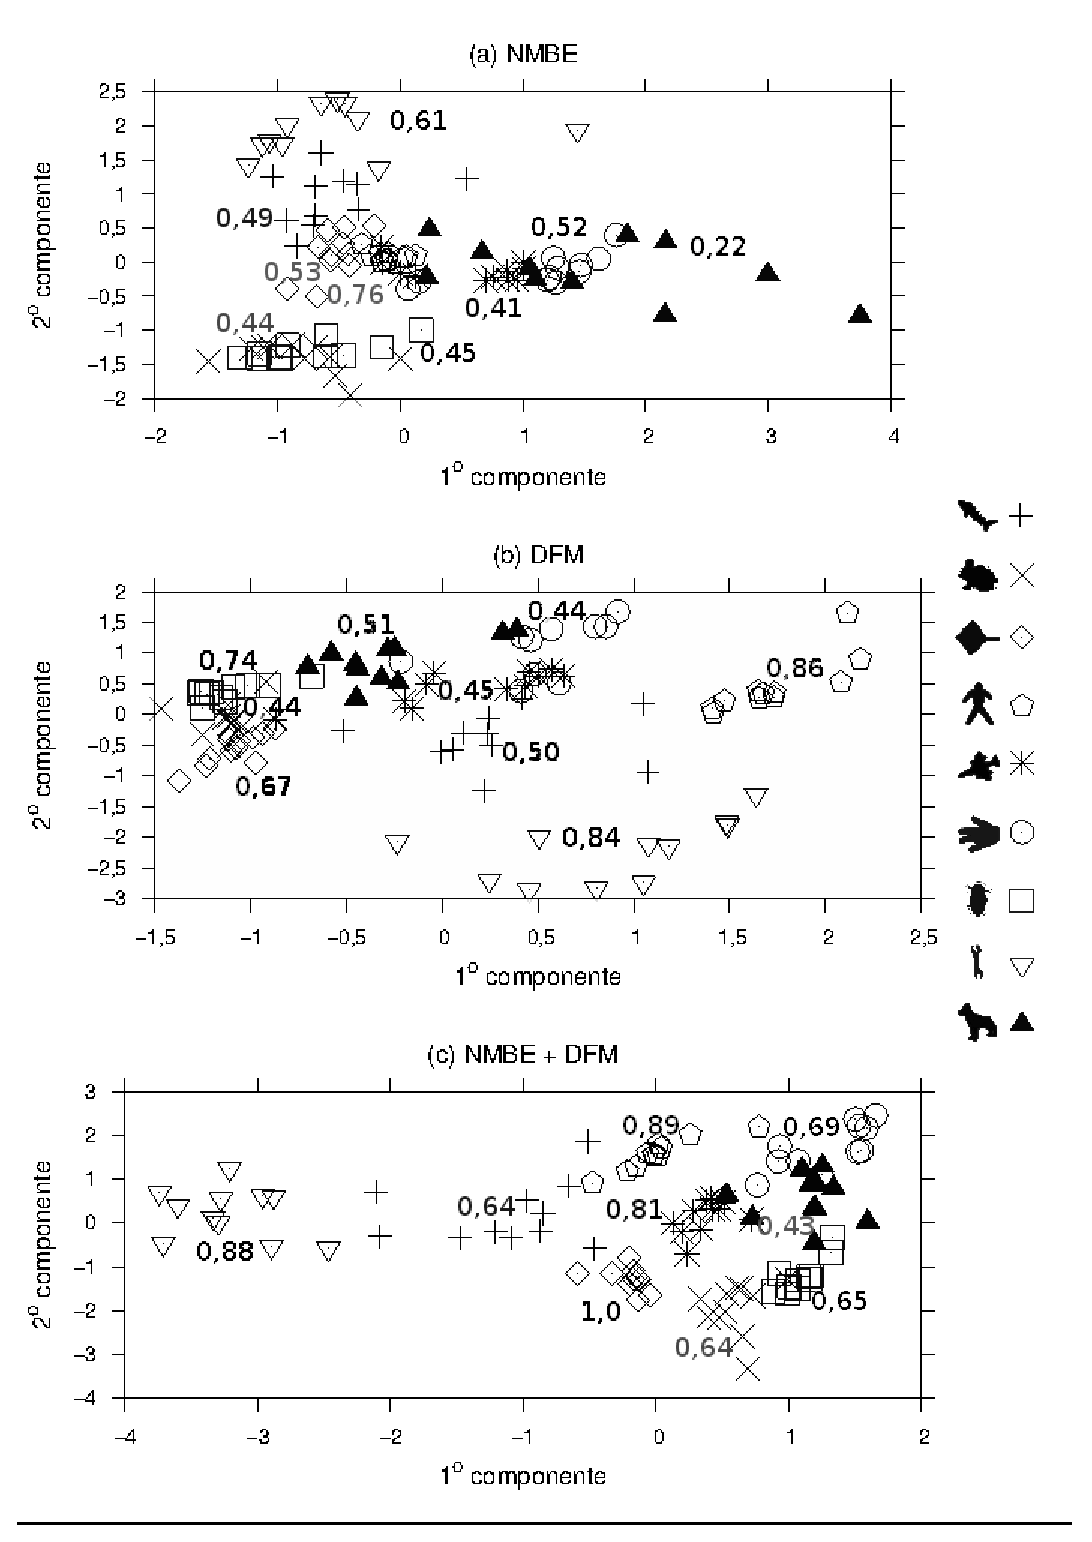
\includegraphics[width=0.75\textwidth]{nuvem_pca.eps}
\end{figure}

\begin{figure}[t]
 \caption{\label{fig:nmbe_dfm_99} Resultados dos descritores NMBE e DFM para a base Kimia-99. (a) Matriz-U obtida com o descritor NMBE e respectiva \textit{Silhouette} média por classe. (b) Matriz-U obtida com o descritor DFM e respectiva \textit{Silhouette} média por classe.}
  \centering
  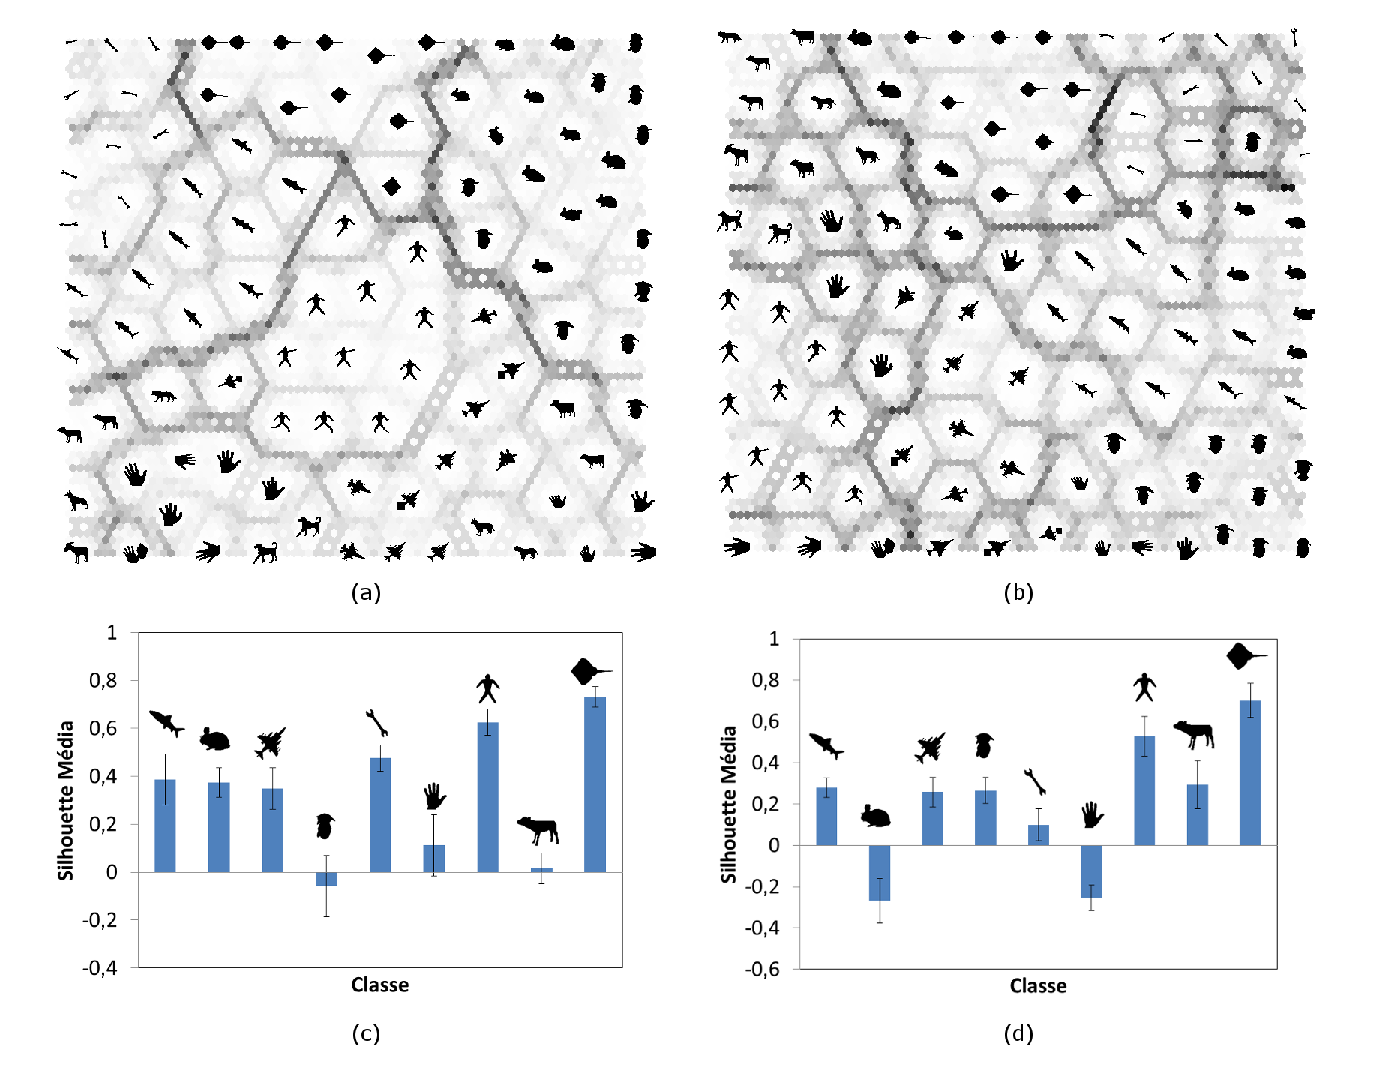
\includegraphics[width=\textwidth]{nmbe_dfm_99.eps}
\end{figure}

\begin{figure}[t]
 \caption{\label{fig:nmbe_dfm_216} Resultados dos descritores NMBE e DFM para a base Kimia-216. (a) Matriz-U obtida com o descritor NMBE e respectiva \textit{Silhouette} média por classe. (b) Matriz-U obtida com o descritor DFM e respectiva \textit{Silhouette} média por classe.}
  \centering
  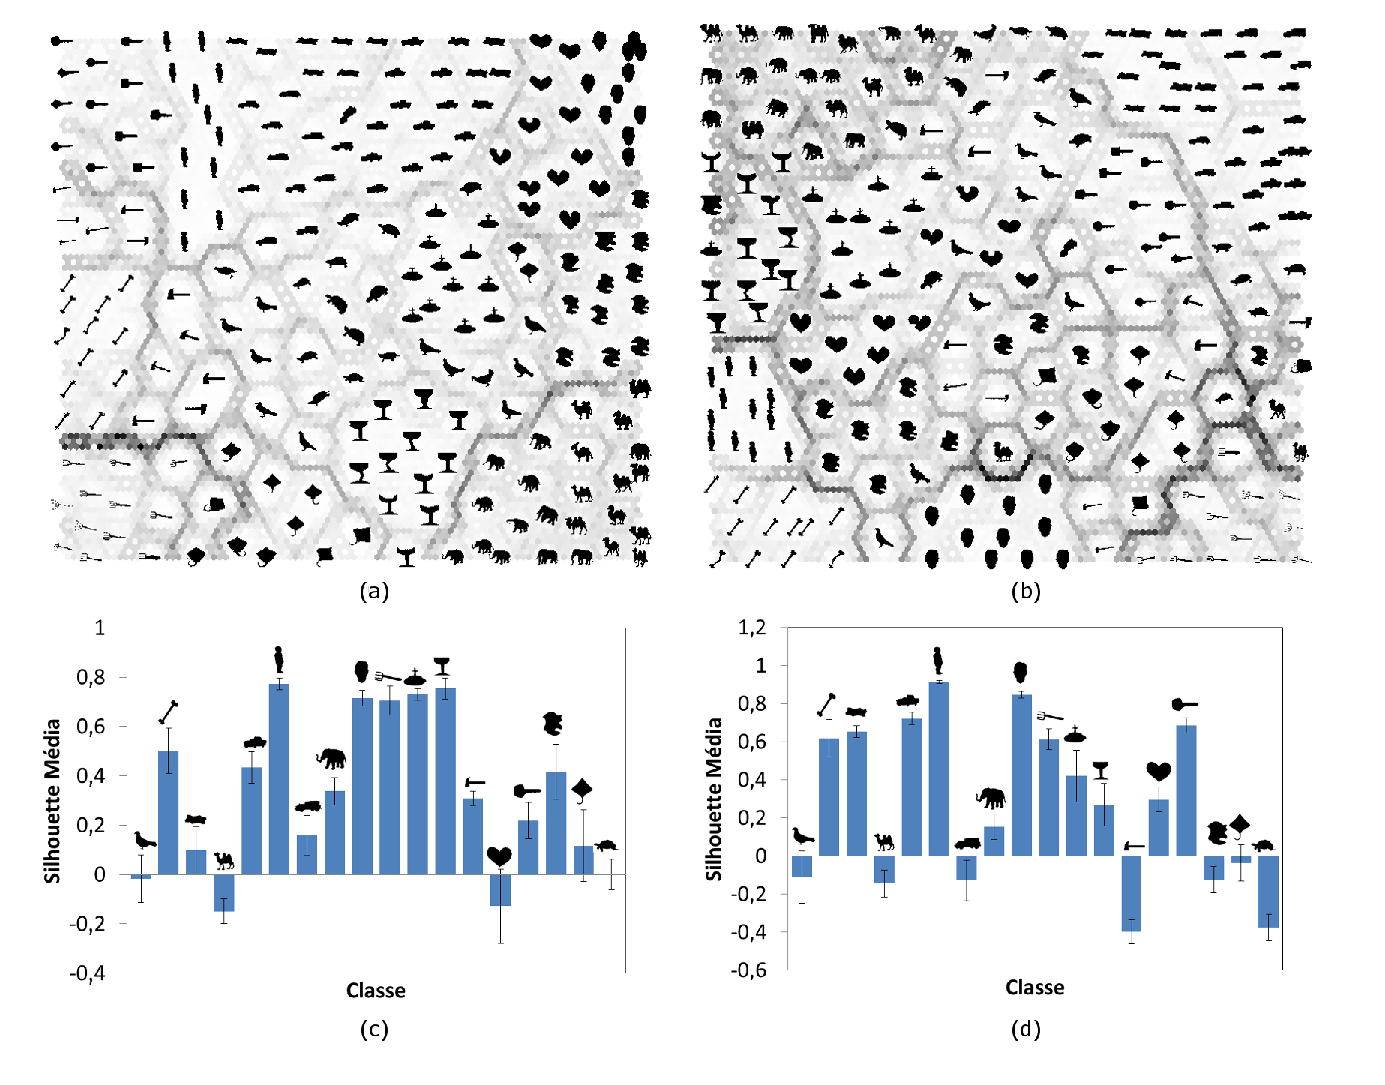
\includegraphics[width=\textwidth]{nmbe_dfm_216.eps}
\end{figure}

Para ilustrar o poder discriminativo dos descritores de forma multiescala NMBE e DFM, bem como mostrar a relação existente entre a medida de avaliação quantitativa da qualidade dos agrupamentos, \emph{silhouette}, e a representação qualitativa obtida através da matriz U, foram realizadas as extrações de características das formas das bases Kimia-99 e Kimia-216 com os referidos descritores. Os resultados estão expostos nas Figuras \ref{fig:nmbe_dfm_99} e \ref{fig:nmbe_dfm_216}. 

Em ambas as figuras, observa-se que as formas correspondentes às classes com  \emph{silhouette} média positiva são visualizadas na matriz-U mantendo forte relação de vizinhança entre si, enquanto que formas correspondentes às classes cuja \emph{silhouette} média é negativa encontram-se dispersas nessas matrizes. Isso denota a inabilidade da descrição  em representa-as adequadamente.

Assim, os descritores conseguem capturar características tanto globais como locais, uma vez que classes de formas com características globais semelhantes, como por exemplo as formas alongadas do canto superior esquerdo da Figura \ref{fig:nmbe_dfm_216}a, estabelecem uma relação de vizinhança entre si. Apesar disso, formas alongadas de classes distintas não se misturam, o que é um indicativo de que o descritor foi capaz também de representar características locais discriminativas que permitem a separação entre as classes.

Existe no entanto,  casos em que ambos os descritores não foram capazes de discriminar formas com características globais semelhantes, como é o caso das classes de formas de elefantes e camelos na Figura \ref{fig:nmbe_dfm_216}. Na matriz-U, estas formas aparecem agrupadas como se pertencessem a uma mesma classe e consequentemente, com valores de \emph{silhouette} média significativamente menores em relação às formas que foram discriminadas corretamente pelos descritores.

A Figura \ref{fig:MatrizU_leaves_256}a mostra a matriz-U obtida para as formas de folhas de plantas da base Flavia representadas pelo descritor NMBE otimizado e a Figura \ref{fig:MatrizU_leaves_256}b, pelo descritor NMBE não otimizado. A análise exploratória visual dos agrupamentos produzidos pela descrição NMBE indica que a descrição otimizada melhora a organização dos agrupamentos. Essa evidência então confirma que a função objetivo MAD é adequada para guiar o processo de otimização desse descritor. A visualização das formas nas matrizes-U da Figura \ref{fig:MatrizU_leaves_256}  aponta diferenças entre os dois arranjos promovidos pelos referidos descritores. A cada posição ou elemento da matriz, os valores numéricos foram substituídos pela imagem das folhas correspondentes, estando as cores das folhas em correspondência com o rótulo das classes exibidas na Figura \ref{fig:bases}. Nessas matrizes-U estão representadas as $1907$ formas de folhas da base Flavia, sendo cada folha representada por sua descrição multiescala.

Os gráficos representativos da \emph{silhouette} média nas  Figura \ref{fig:MatrizU_leaves_256}a  e Figura \ref{fig:MatrizU_leaves_256}b demonstram que as classes das folhas bem caracterizadas e, portanto, agrupadas adequadamente são as que apresentam valores de \emph{silhouette} média positivos. Por outro lado, as classes de folhas que o descritor não foi capaz de caracterizar e agrupar adequadamente são as que apresentaram valores negativos de \emph{silhouette} média. Comparando estes resultados, observa-se que na Figura \ref{fig:MatrizU_leaves_256}a há expressiva redução dos valores negativos de \emph{silhouette} média quando se utiliza o descritor $\operatorname{NMBE_{opt}}$. 

\begin{figure}[t]

\caption{\label{fig:MatrizU_leaves_256} Matrizes-U e a \emph{silhouette} média para as descrições das folhas da base Flavia com o descritor NMBE (a) optimizado e (b) não otimizado.}
\centering
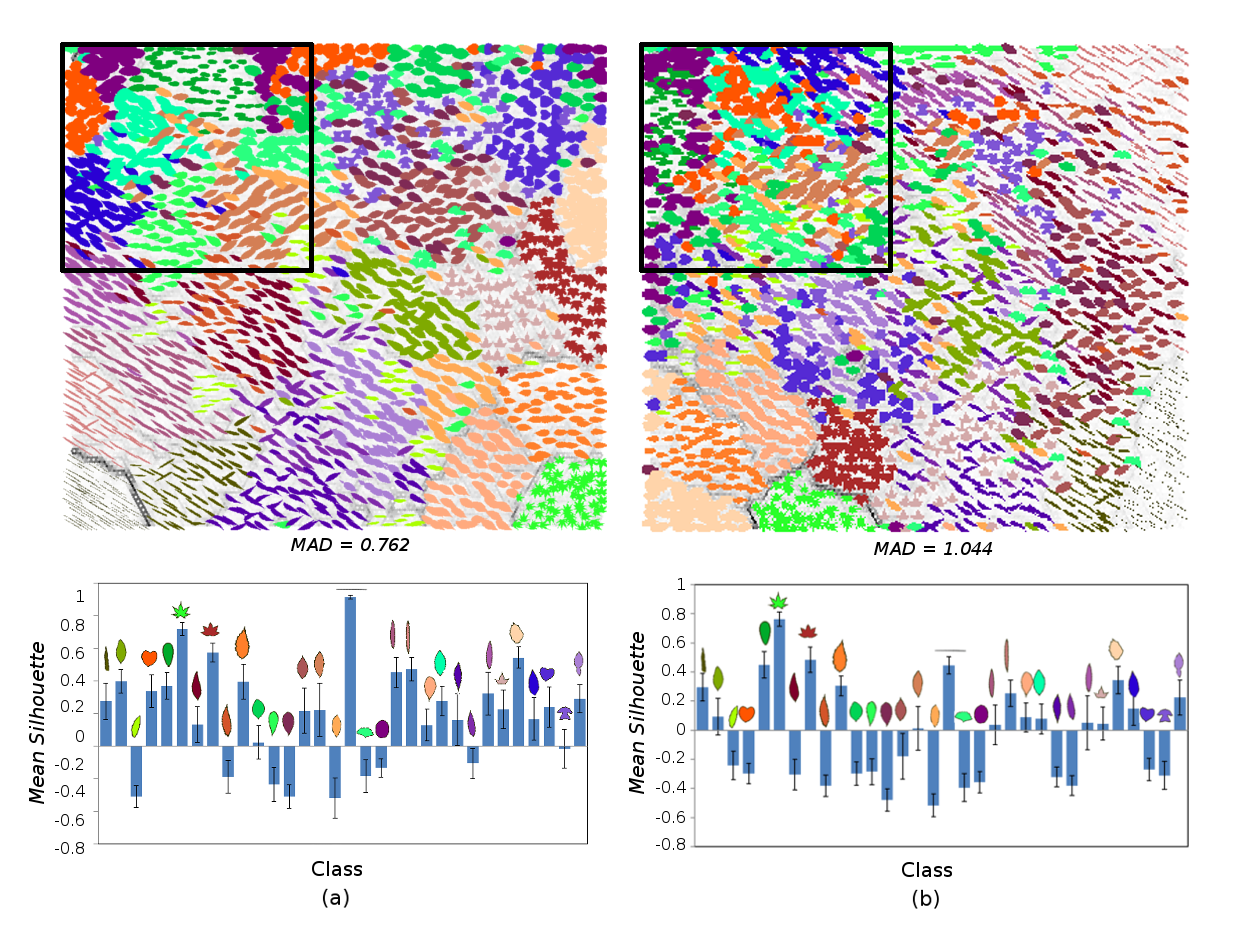
\includegraphics[width=\textwidth]{fig7.eps}

\end{figure}

O quadrado preto inserido na Figura \ref{fig:MatrizU_leaves_256} destaca o desempenho do descritor otimizado em termos de melhoria no arranjo das formas na matriz-U. É possível ainda observar quão bem o descritor otimizado mapeou as folhas em grupos de acordo com as respectivas classes rotuladas das mesmas.  Além do mais, o resultado com as escalas otimizadas melhorou significativamente a \emph{silhouette} média por classe para quase todas as classes de folhas da base. Por outro lado, a região interna ao quadrado preto na Figura \ref{fig:MatrizU_leaves_256}b destaca que o descritor não otimizado não foi capaz de mapear satisfatoriamente as formas de  folhas em suas classes correspondentes. Deduzimos que essa melhoria se deve ao fato de que as escalas otimizadas dos descritores são mais sensíveis a variações intrínsecas das formas, ou sejam, incorporam nuances presentes nos seus contornos, os quais os métodos tradicionais não o fazem adequadamente. Além do mais, o ajuste automático das escalas é de fato uma tarefa alternativa para o ajuste arbitrário ou empírico, sendo que esta última não é uma tarefa simples e está sujeita à fadiga e subjetividade do realizador da mesma.


As Figuras \ref{fig:MatrizU_leaves_II}a, \ref{fig:MatrizU_leaves_II}b and \ref{fig:MatrizU_leaves_II}c exibem as matrizes-U correspondentes aos valores MAD dos experimentos na base Flavia utilizando os algoritmos de otimização SA, DE e PSO, respectivamente. Um aspecto interessante a examinar é o fato dos três algoritmos apresentarem diferentes soluções, ou valores de MAD. Estas soluções resultaram em diferentes arranjos de folhas e consequentemente diferentes relações entre as estruturas de vizinhança dos grupos ou classes.
Por exemplo, a dispersão geral dos elementos nas Figuras \ref{fig:MatrizU_leaves_II}a e \ref{fig:MatrizU_leaves_II}b tende a ser muito semelhante uma vez que seus respectivos valores da função objetivo minimizada são bem próximos em magnitude. Ao mesmo tempo, concluímos que o resultado que corresponde ao mais elevado valor de MAD ($0,829$) exibe uma dispersão particularmente elevada no centro da Matriz-U (Figura \ref{fig:MatrizU_leaves_II}c). Este é um detalhe que reforça a observação anterior de que o PSO convergiu para um mínimo local. 
Estes achados apontam para a importante conclusão de que quanto menor o valor de MAD, melhor o arranjo dos grupos ou do agrupamento, e consequentemente a qualidade do agrupamento. Por isso, afirmamos que a qualidade dos grupos e o valor de MAD são negativamente correlacionados. Nossa análise ainda considera que devam existir outras soluções no espaço de busca, além da solução mínima, que sejam adequadas ao problema em estudo.

\begin{figure}[h!] \caption{\label{fig:MatrizU_leaves_II}Matrizes-U e valores MADs obtidos para a base de imagens Flavia por uso da NMBE otimizada pelos algoritmos (a) SA, (b) DE, (c) PSO.}
\centering
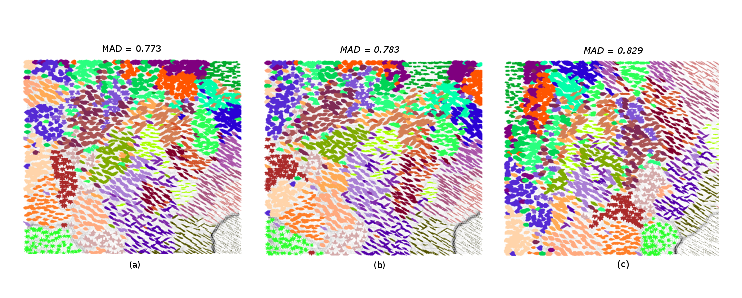
\includegraphics[width=\textwidth,trim = 0mm 0mm 0mm 4.5mm,clip]{fig8.eps}
\end{figure}

A Figura \ref{MDS:Leaves} ilustra as projeções MDS para três valores distintos de MAD. Na Figura \ref{MDS:Leaves}a temos o arranjo dos agrupamentos após a convergência do algoritmo de otimização SA, ou seja, para o descritor cujos parâmetros otimizados correspondem ao mínimo valor da função MAD encontrado nas otimizações. Analisando essas projeções, observa-se que a minimização da função objetivo resultou em agrupamentos de folhas com maior coesão intra classe e maior separação entre classes. A análise visual das três regiões detalhadas  nessa imagem indica mais claramente que o descritor NMBE otimizado melhorou a representação das formas de folhas em comparação aos resultados das Figuras \ref{MDS:Leaves}b e \ref{MDS:Leaves}c. Ademais, os valores do coeficiente $R^2$ próximos de $1,0$ indicam que a representação no espaço bi-dimensional preservou a relação de distâncias entre as amostras no espaço de alta dimensão.

\begin{figure}[t]
 \caption{\label{MDS:Leaves} Projeções MDS dos descritores NMBE para formas da base de folhas Flavia. (a) Descritor NMBE otimizado pelo algoritmo SA com valor de função $MAD = 0,762$ (b) Descritor NMBE não otimizado com valor de função $MAD =0,969$ and (c) Descritor NMBE não otimizado com valor de função $MAD = 1,044$.}

\centering
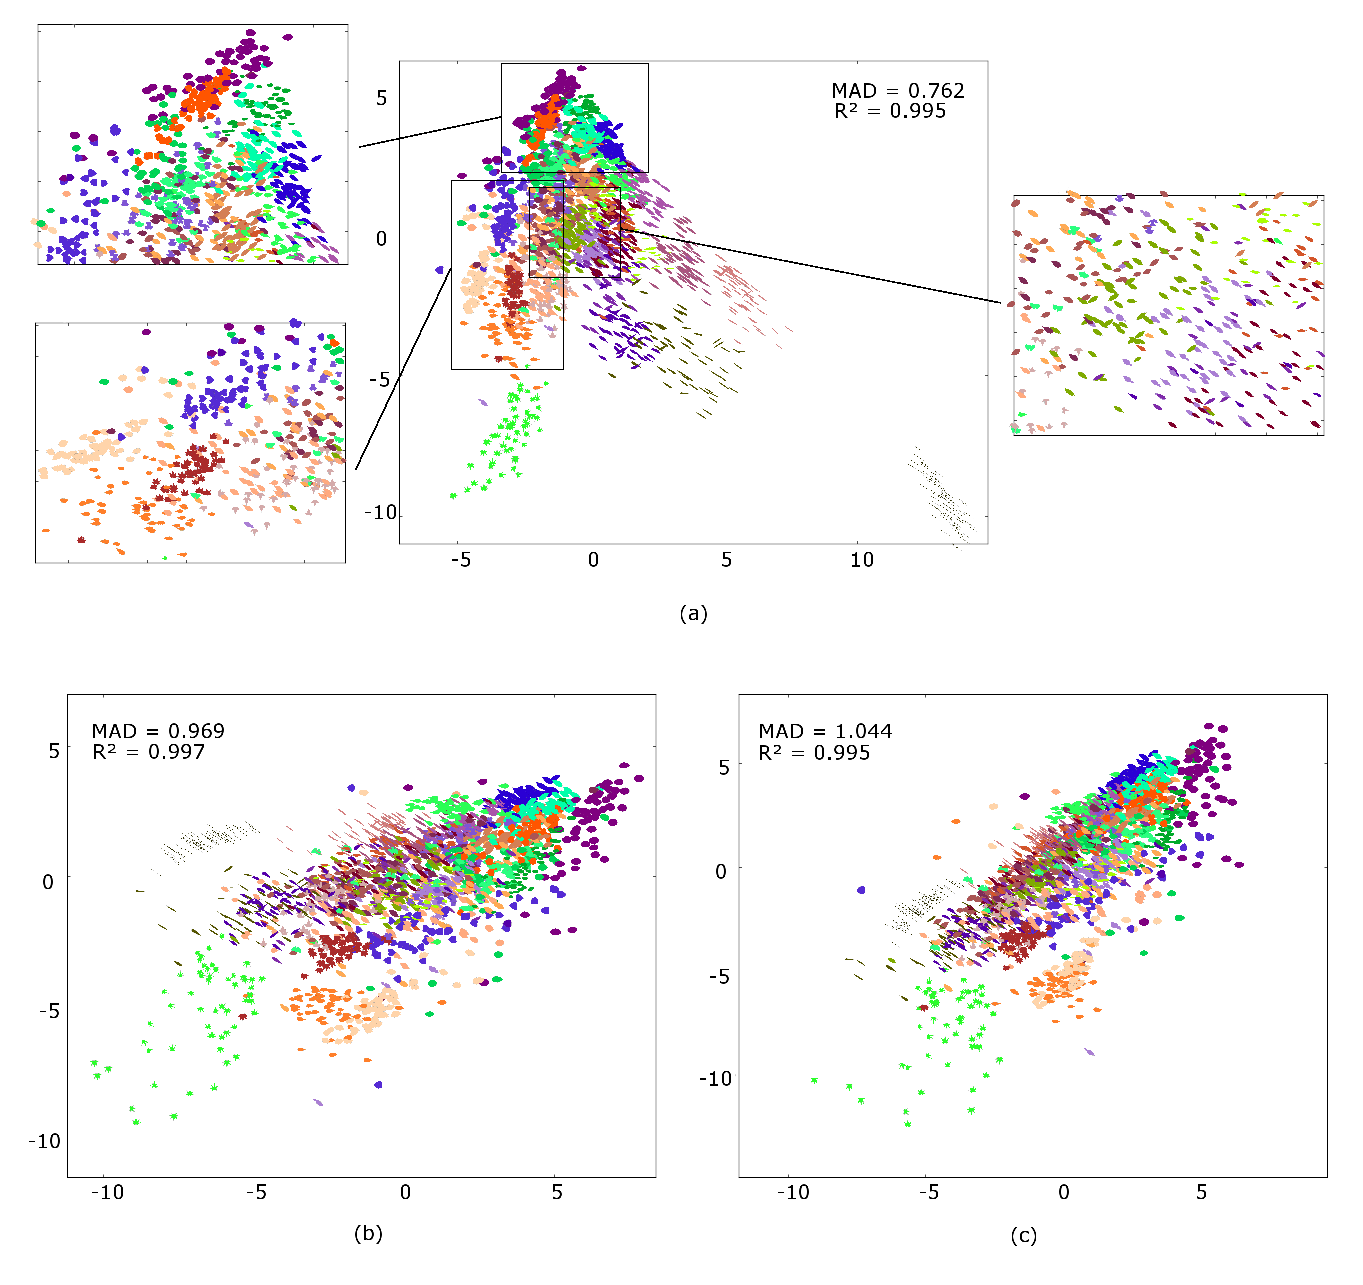
\includegraphics[width=0.7\textwidth]{fig9.eps}
\end{figure}

\section{Recuperação de imagens baseada em conteúdo - CBIR}

O descritor IDSC \cite{Ling:2007:SCU:1191552.1191806} foi otimizado para fins de comparação com o descritor multiescala. Desenvolvido para aplicações de recuperação de formas, o IDSC utiliza algoritmos de programação dinâmica, tal como o DTW \cite{PalazonGonzalez2012978}, para melhorar a precisão da avaliação de similaridade entre formas. Assim sendo, subsituimos a norma $L_2$ pelo algoritmo DTW no cálculo da medida \emph{silhouette}, uma vez que esta última é requerida para a avaliação da função objetivo MAD na Equação \ref{eq:mad}. 

A Figura \ref{fig1Ooptimization_graph}a exibe gráficos que permitem a comparação dos resultados dos experimentos realizados para as versões otimizadas ($\operatorname{NMBE_{opt}}$, $\operatorname{IDSC_{opt}}$)
 e não otimizadas ($\operatorname{NMBE}$, $\operatorname{IDSC}$) de ambos descritores. Os gráficos mostram que o ajuste dos parâmetros dos descritores pelo método de otimização melhorou o resultado (taxa) de recuperação de folhas consideravelmente. Observamos ainda que o descritor $\operatorname{IDSC_{opt}}$ superou ambos os descritores $\operatorname{NMBE_{opt}}$ e NMBE não otimizado com relação à taxa de recuperação. Logo, podemos afirmar que a otimização de parâmetros melhorou a capacidade de discriminação do  $\operatorname{IDSC_{opt}}$, incorporando ao descritor um mecanismo de extração de informações relevantes de detalhes intrínsecos das formas das folhas. Por outro lado, observamos que o desempenho do IDSC não otimizado foi inferior ao do NMBE não otimizado. 

As Figuras \ref{fig1Ooptimization_graph}b e \ref{fig1Ooptimization_graph}c ilustram resultados obtidos de recuperação de dois exemplares da base de imagens de folhas para experimentos realizados com os descritores NMBE não otimizado e $\operatorname{NMBE_{opt}}$,  IDSC não otimizado com parâmetros ajustados conforme recomendado em \cite{wang2015march} e $\operatorname{IDSC_{opt}}$. Observa-se na Figura \ref{fig1Ooptimization_graph}b que o descritor NMBE não otimizado falhou parcialmente na recuperação das formas, enquanto a versão otimizada ($\operatorname{NMBE_{opt}}$) com sucesso recuperou todas as formas. O mesmo comentário se aplica ao descritor $\operatorname{IDSC_{opt}}$, cujos resultados mostram o sucesso da recuperação. Ainda na Figura \ref{fig1Ooptimization_graph}c, o descritor IDSC não otimizado não foi capaz de recuperar as amostras corretamente.

\begin{figure}[]
\caption{Experimentos realizados com formas da base de imagens de folhas Flavia (a) taxa de recuperação  obtida com os descritores NMBE e IDSC originais e suas versões otimizadas, (b) e (c) recuperação de duas amostras de folhas utilizando os descritores NMBE e IDSC otimizados e não otimizados, respectivamente.\label{fig1Ooptimization_graph}}
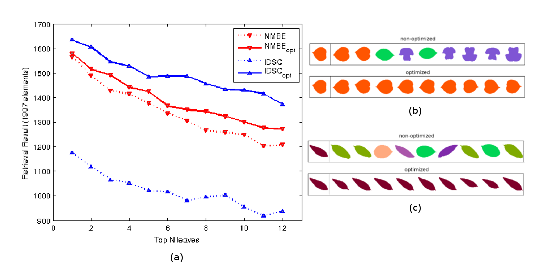
\includegraphics[width=\textwidth]{fig10.eps}
\end{figure}

\begin{comment}
\begin{figure}[t!]
\begin{subfigure}{0.55\textwidth}
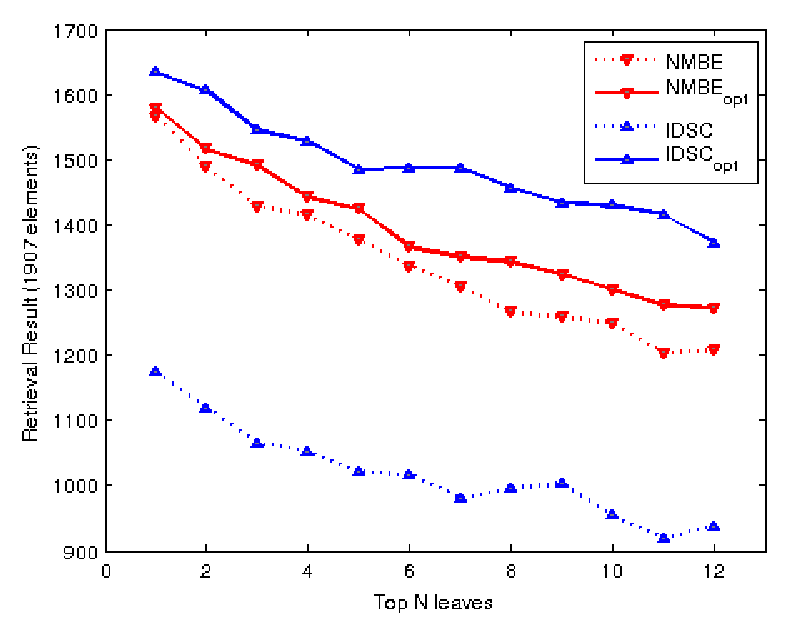
\includegraphics[width=\textwidth]{fig10a.eps}
\caption{Retrieval rates. \label{fig1Ooptimization_graph}}
\end{subfigure}
\hspace*{\fill}
\begin{minipage}{0.45\textwidth}
\begin{subfigure}{\textwidth}
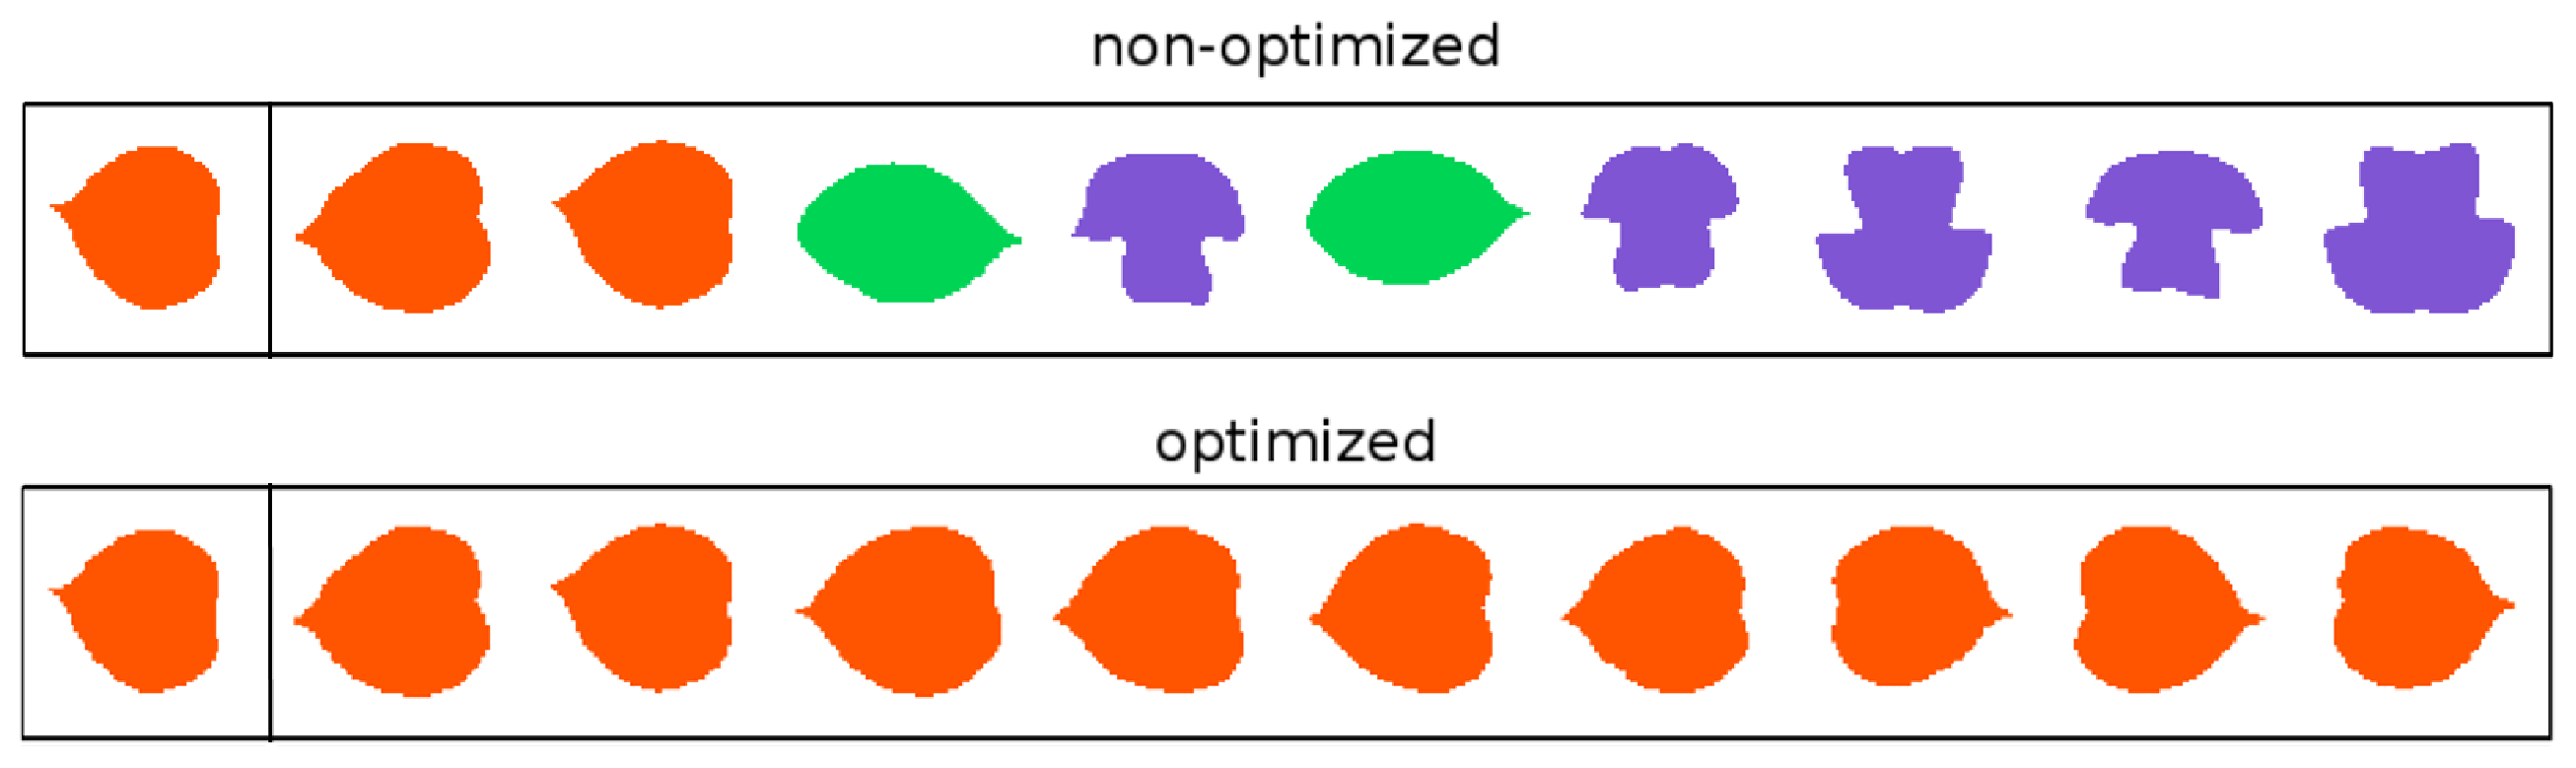
\includegraphics[width=\textwidth]{fig10b.eps}
\caption{Retrieval results with NMBE.} \label{subfig:upper-right}

\end{subfigure}

\vspace*{0.60cm}
\begin{subfigure}{\textwidth}
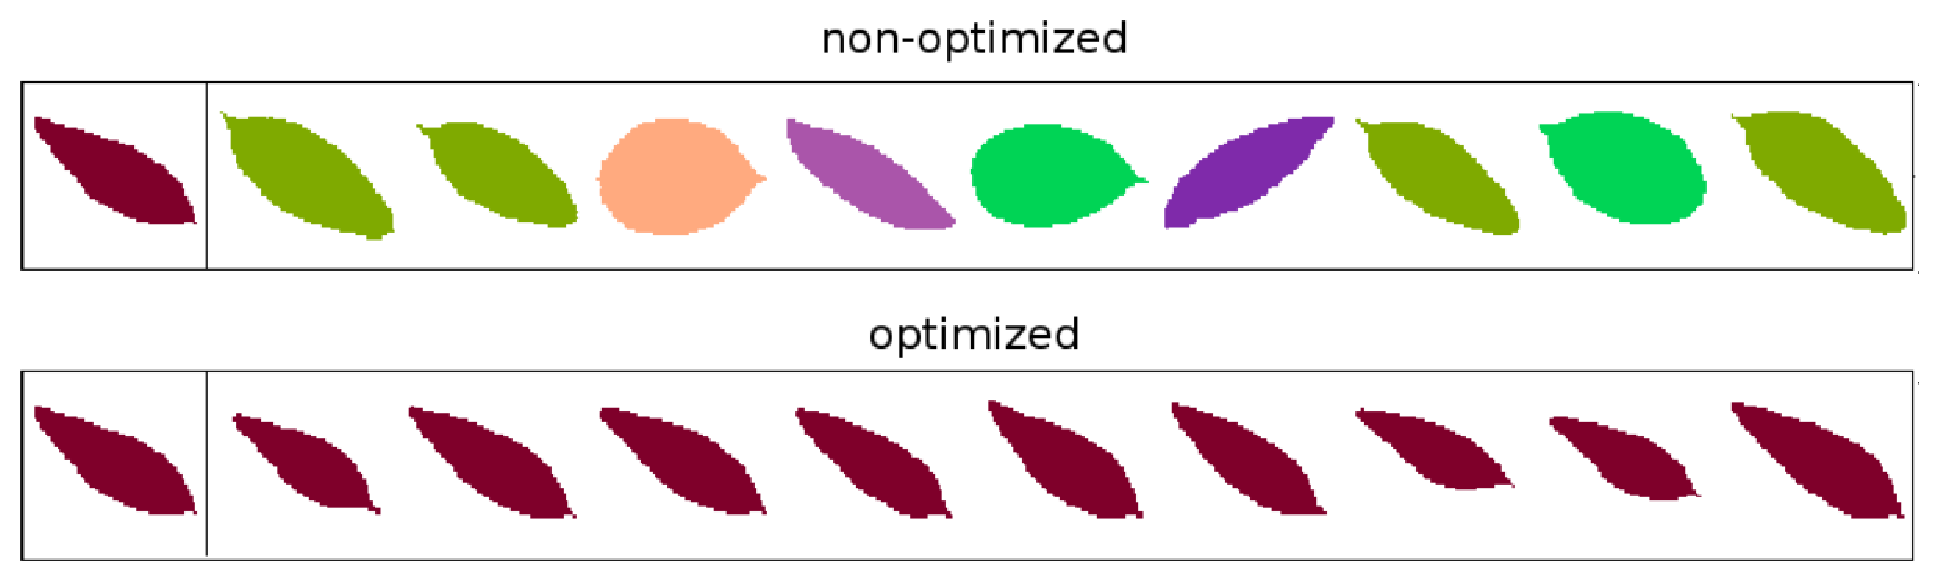
\includegraphics[width=\textwidth]{fig10c.eps}
\caption{Retrieval results with IDSC.\label{subfig:lower-right}}
\end{subfigure}
\end{minipage}

\caption{\label{figfig1Optmization-IDSC} Experiments conducted on Flavia leaf data set (a) retrieval rate by using both NMBE and IDSC and their optimized counterparts, (b) and (c) two leaf shape retrieval examples by using the non-optimized and optimized NMBE and IDSC descriptors, respectively.} 
\end{figure}
\end{comment}

A Tabela \ref{table_bull_eyes_leaves} apresenta o resultado da avaliação de desempenho dos descritores $\operatorname{NMBE_{opt}}$ e NMBE não otimizado com escalas ajustadas conforme recomendado em \cite{Cesar:1996},  $\operatorname{IDSC_{opt}}$ e o IDSC não otimizado. Esses resultados mostram que a taxa de recuperação para ambos os descritores otimizados superou os resultados dos pares correspondentes não otimizados. A melhoria significativa observada nas medidas Bulls-eye reforça a hipótese de que a metodologia de otimização proposta é adequada para ajuste dos descritores em aplicações de recuperação e análise de formas de folhas.

\begin{table}[h!]
\centering
\caption{Taxa Bulls-eye para a base de imagens Flavia.}
\label{table_bull_eyes_leaves}
  \begin{tabular}{cccccccc}
  \toprule[1.5pt]
 $\operatorname{NMBE}$ & $\operatorname{NMBE_{opt}}$ & IDSC    & $\operatorname{IDSC_{opt}}$\\ \midrule
     63.86 \%  & 71.16 \%  & 53.38\%    & 77.50\%       \\
  \bottomrule[1.5pt]
  \end{tabular}
\end{table}

\section{Custo computacional da otimização \label{sec:comp_cost}}


 Nesta tese avaliamos a complexidade computacional dos três algoritmos de otimização como exibe a Tabela \ref{tbl:complexity}.  Os algoritmos SA e PSO apresentam complexidades similares e estas dependem do número de iterações para convergir ($N_{iter}$), do tamanho da população  ($N_{pop}$) e do parâmetro $P$.  Por outro lado, o algoritmo DE demanda maior complexidade, pois depende da dimensão ($D$) do problema a ser otimizado, do tamanho da população ($N_{pop}$) e do número de interações ($N_{iter}$).

\begin{table}[h!]
\centering
\caption{Complexidade computacional dos métodos de otimização.}
\label{tbl:complexity}
  \begin{tabular}{ll}
  \toprule[1.5pt]
 Método & Complexidade\\
 \midrule
   SA  & $O(P.N_{iter}.\log{N_{iter}})$    \\
   DE  & $O(N_{pop}.N_{iter}.D)$   \\
   PSO&  $O(N_{pop}.N_{iter}.\log{N_{iter}})$\\
  \bottomrule[1.5pt]
  \end{tabular}
\end{table}

Para fins de comparação dos métodos de otimização, sob o aspecto de custo computacional, assumimos o custo computacional dos algoritmos como sendo o número de vezes que a função objetivo é demandada ao longo do processo de otimização. Considerando para cada método de otimização o ajuste de parâmetros adotado, bem como a complexidade computacional correspondente, os custos computacionais calculados para os algoritmos SA, DE e PSO resultaram em $7.4314$, $19.500$ e $1.107$, respectivamente. 

Vale destacar que existe um compromisso entre o custo computacional e a qualidade da solução ótima obtida. Assim sendo a redução do número de amostras de formas, da resolução das imagens e do tamanho da população dos métodos ($N_{pop}$) ameniza o custo computacional, porém estas reduções degradam a qualidade do resultado da otimização. Ademais, o uso de processamento paralelo pode contribuir para a redução do custo computacional, sem degradar a qualidade da solução ótima, entretanto o paralelismo adiciona complexidade aos algoritmos de otimização. 



\begin{comment}
\begin{figure}
 \caption{\label{fig:edif99} (a) Matriz-U para as formas da base Kimia99 representadas com o descritor entropia multiescala. (b) Silhouette média por classe aferida a partir do descritor}
  \centering
  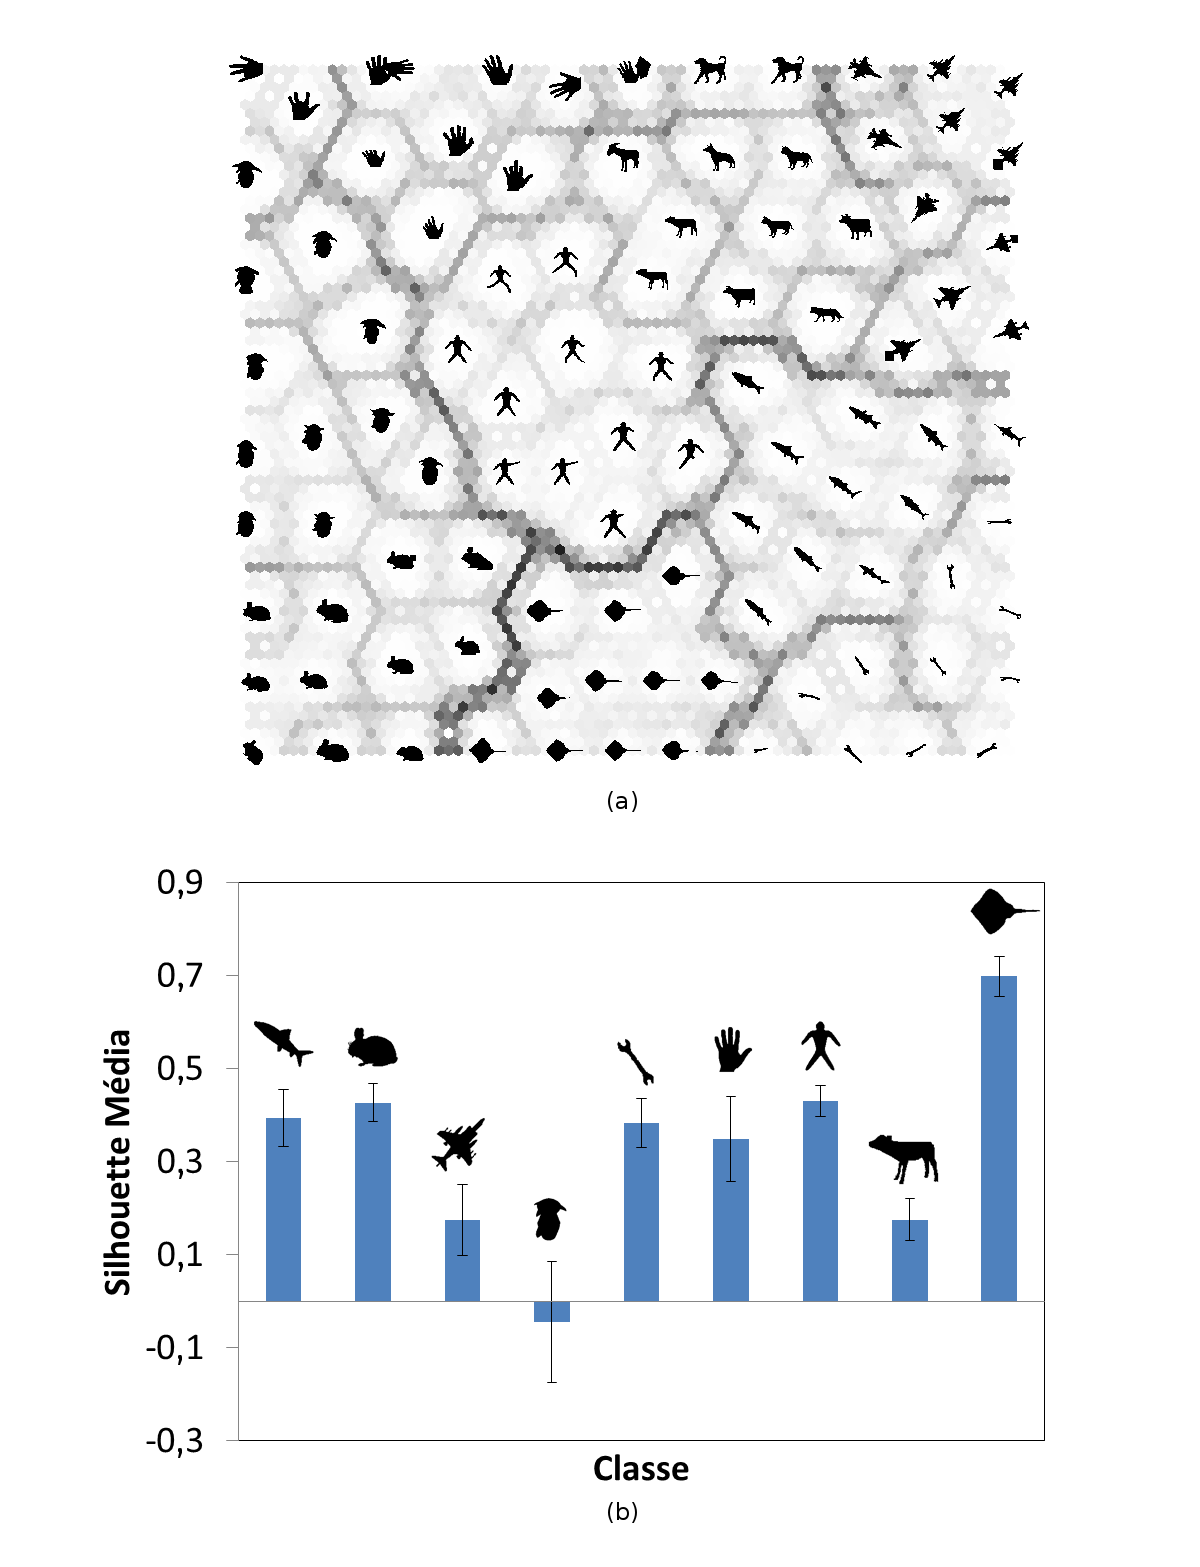
\includegraphics[width=\textwidth]{ediferencial99.png}
\end{figure}

\begin{figure}
 \caption{\label{fig:edif216} (a) Matriz-U para as formas da base Kimia216 representadas com o descritor entropia multiescala. (b) Silhouette média por classe aferida a partir do descritor}
  \centering
  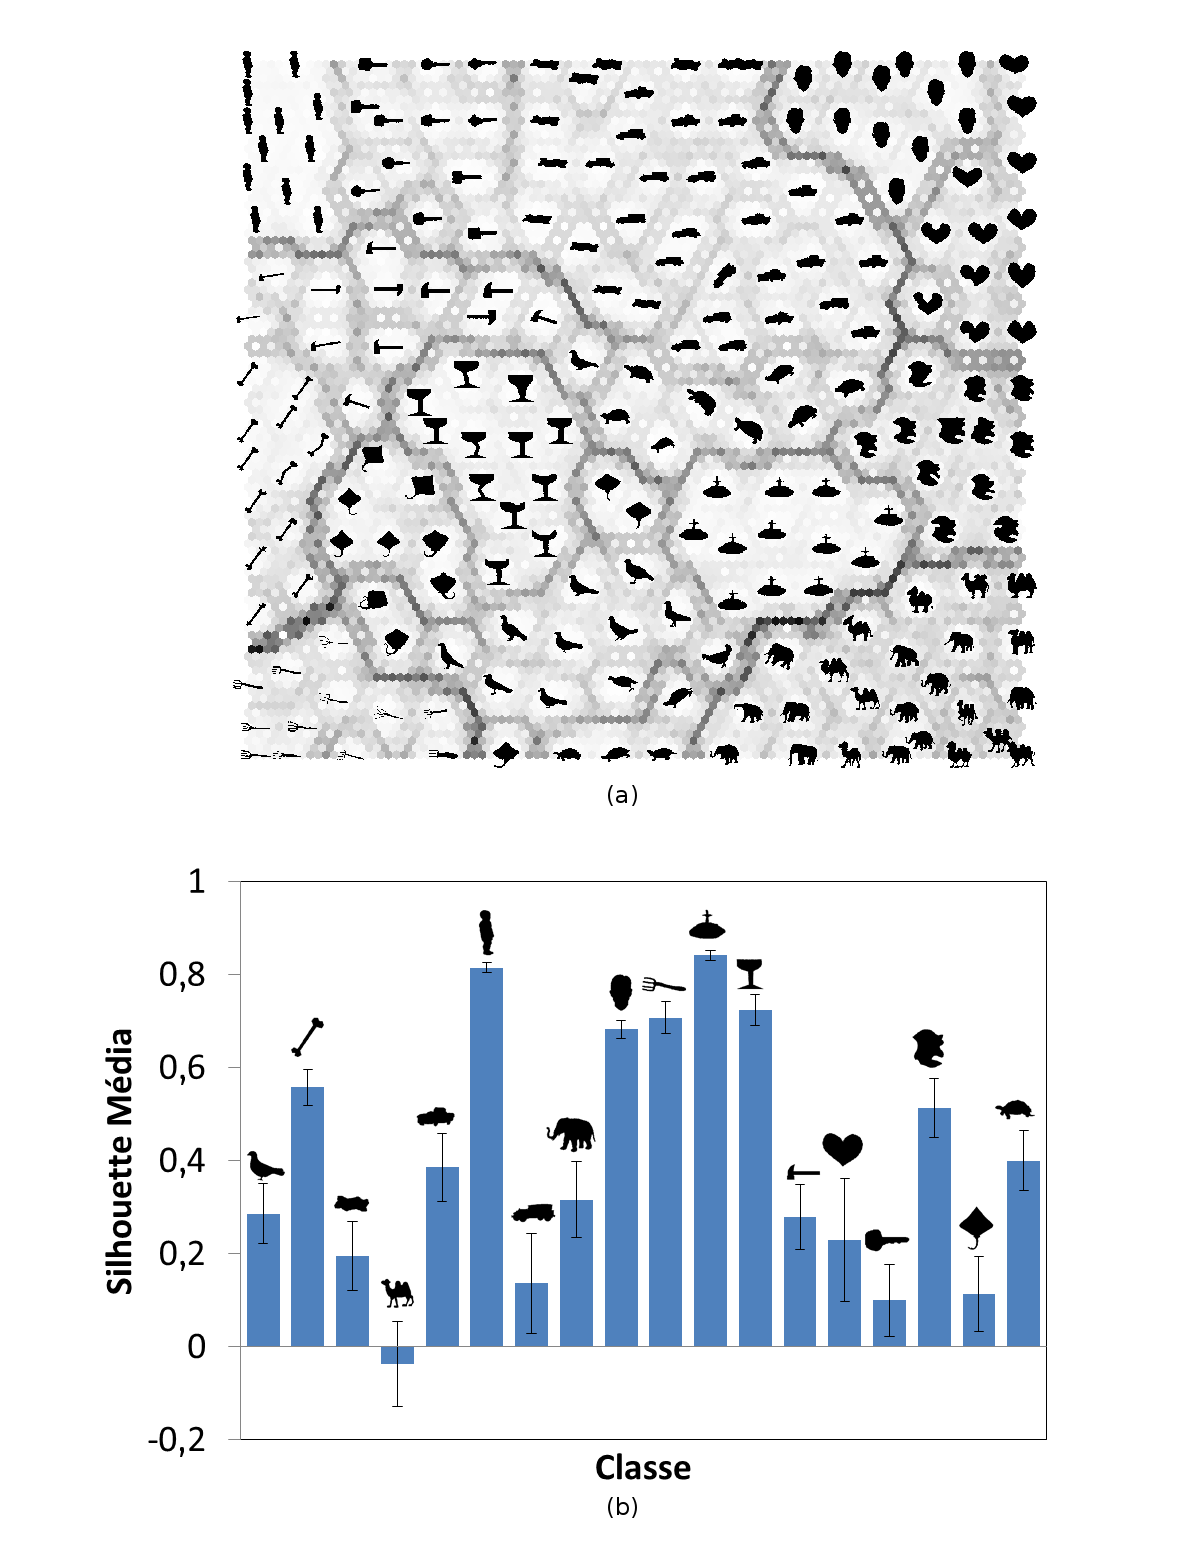
\includegraphics[width=\textwidth]{ediferencial216.png}
\end{figure}

\begin{figure}
 \caption{\label{fig:edis99} (a) Matriz-U para as formas da base Kimia99 representadas com o descritor entropia multiescala. (b) Silhouette média por classe aferida a partir do descritor}
  \centering
  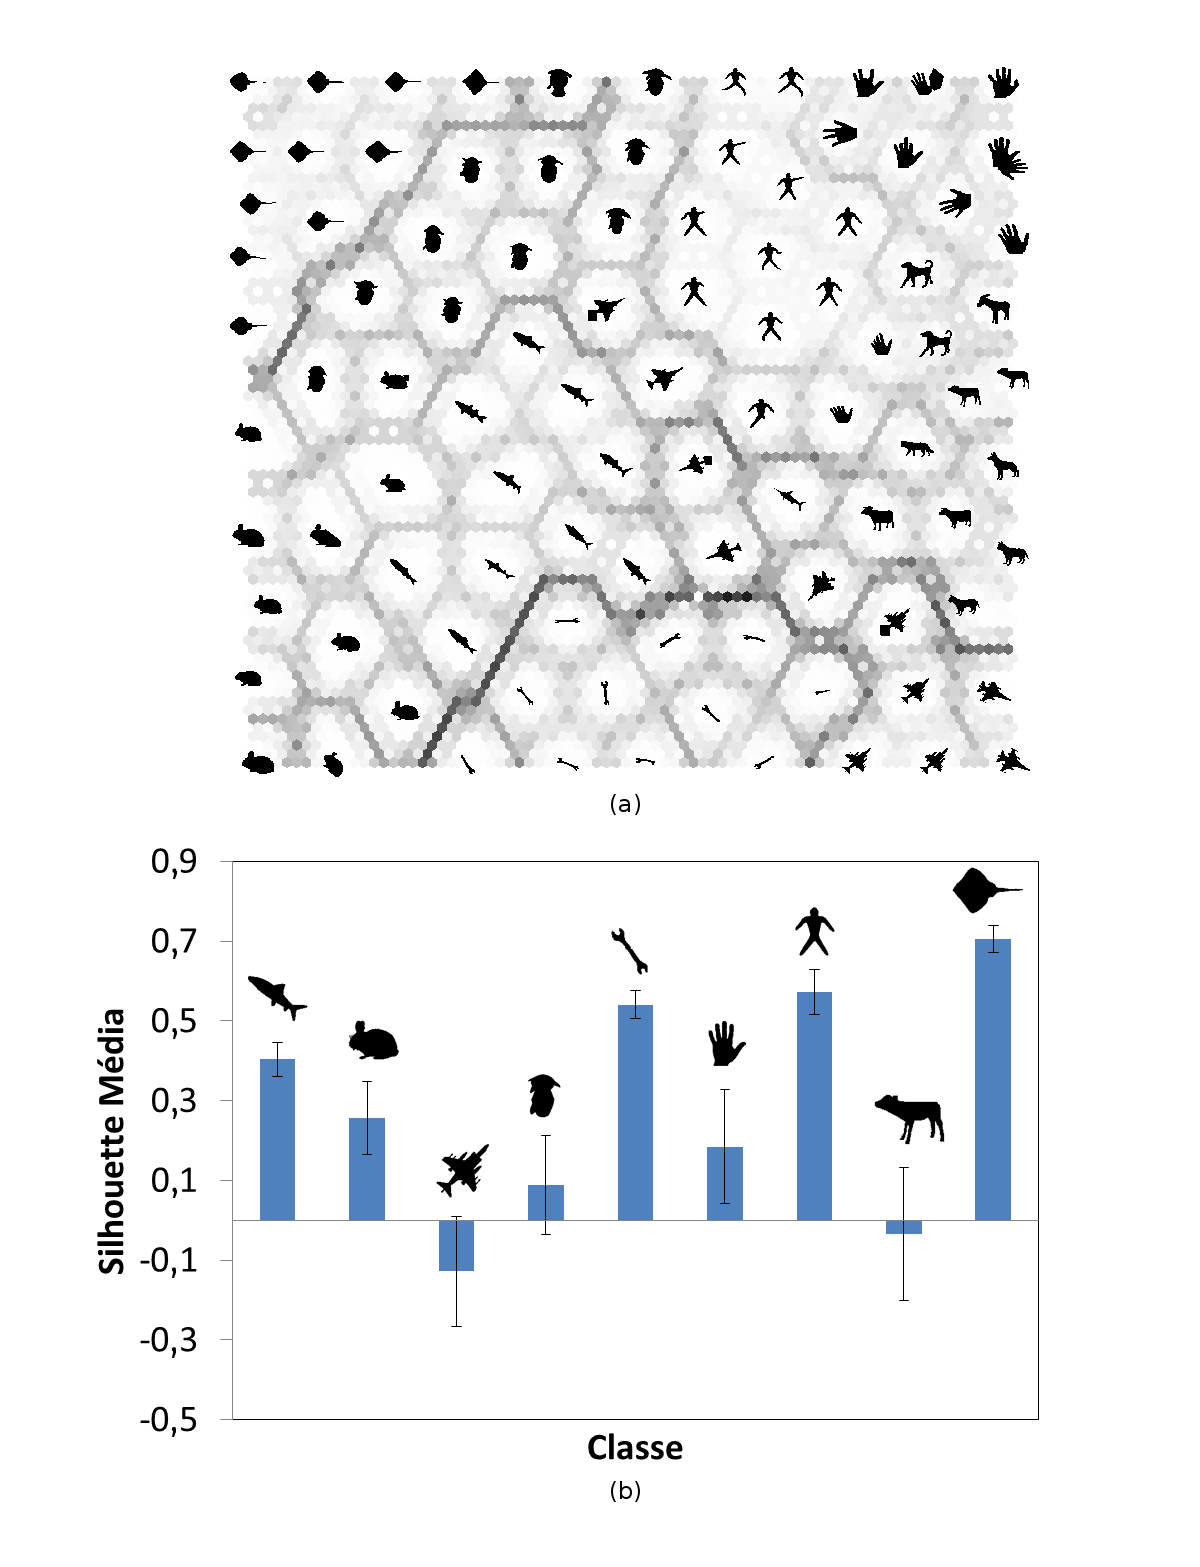
\includegraphics[width=\textwidth]{ediscreta99.png}
\end{figure}

\begin{figure}
 \caption{\label{fig:edis216} (a) Matriz-U para as formas da base Kimia216 representadas com o descritor entropia multiescala. (b) Silhouette média por classe aferida a partir do descritor}
  \centering
  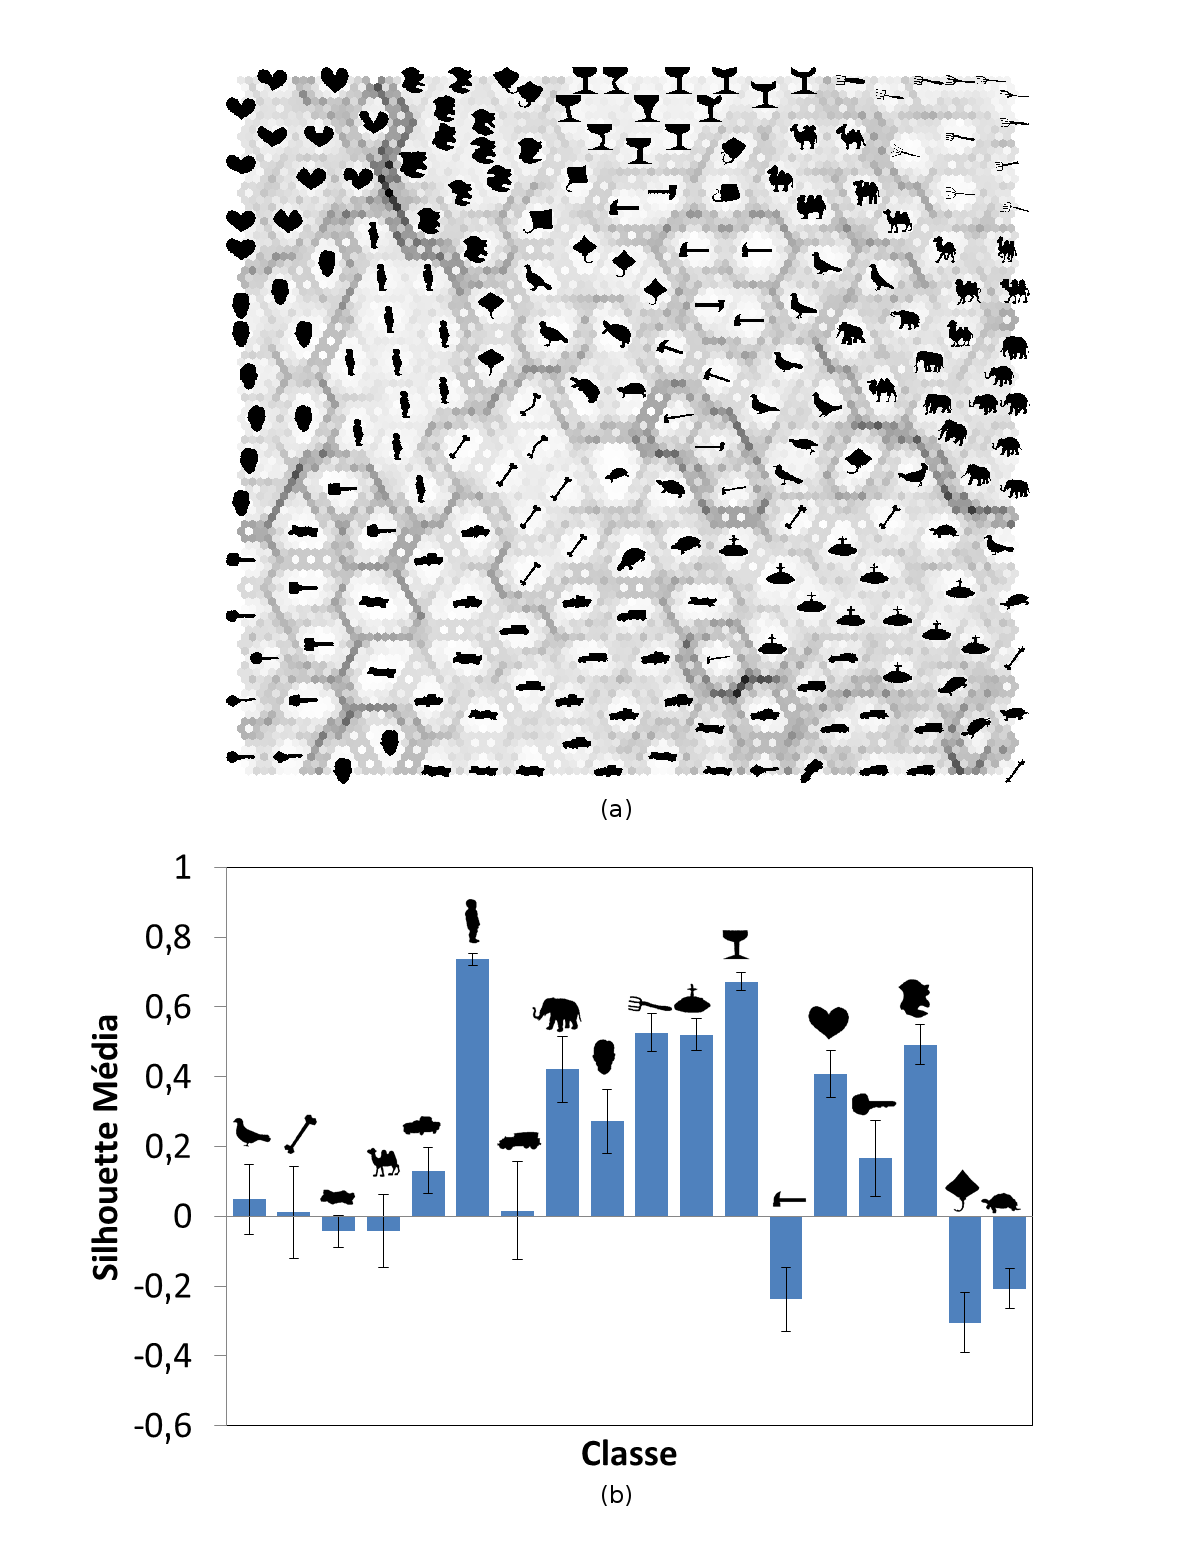
\includegraphics[width=\textwidth]{ediscreta216.png}
\end{figure}

\subsection{\emph{NMBE} e \emph{DFM}}
Os experimentos de avaliação de desempenho dos descritores produziram como saída as matrizes-U que estão apresentadas na Figuras \ref{fig:nmbe_som_map}, \ref{fig:mfd_som_map} e  \ref{fig:som_kimia_216}. Nas Figuras \ref{fig:nmbe_som_map} e \ref{fig:mfd_som_map}, as regiões delimitadas com linhas tracejadas correspondem as classes de formas com os maiores valores médios da medida Silhouette (Figuras \ref{fig:silhouette}a e \ref{fig:silhouette}b). Nesses casos pode-se deduzir que ambos os descritores foram capazes de caracterizar corretamente estas classes de formas.

Já os grupos delimitados com linhas contínuas referem-se às classes de formas com os menores valores de Silhouette média. De fato, as formas dessas classes aparecem nas matrizes-U dispersas em sub-grupos, que é um indicativo que ambos os descritores falharam em caracterizá-las adequadamente.
  
As Figuras \ref{fig:dude_tool_mfd} e \ref{fig:dude_tool_nmbe} mostram objetos das classes de formas de humanos e ferramentas. Ambos os descritores foram capazes de discriminar os objetos das referidas classes, como evidenciado nos gráficos apresentados. As matrizes-U (Figuras \ref{fig:nmbe_som_map} e \ref{fig:mfd_som_map}) também confirmam esse resultado exibindo, para essas classes de formas, homogeneidade intra-classe e separabilidade inter-classes. Logo, concluímos que estes descritores são efetivos em representar formas para o reconhecimento de padrões em aplicações \emph{CBIR}.

Também evidenciamos nas Figuras \ref{fig:mfd_som_map} e \ref{fig:nmbe_som_map} que o descritor \emph{DFM} apresentou maior dispersão inter-classe para as formas de humanos que o descritor \emph{NMBE}. Essa observação é consistente com os resultados obtidos através da medida \emph{Silhouete}, aonde o valor dessa medida para formas humanas descritas com a \emph{DFM} é menor do que o valor para essas mesmas formas descritas com a \emph{NMBE}.

Ademais, os sinais em linhas tracejadas vermelhas e em linhas contínuas azuis, apresentados nas Figuras \ref{fig:dude_tool_mfd} e \ref{fig:dude_tool_nmbe}, mostram que o descritor \emph{NMBE} é mais robusto a diferenças intra-classe que o descritor \emph{DFM}. Nesses gráficos, as formas pertencentes a mesma classe que o descritor representa seguindo um mesmo padrão apresentam-se próximas umas das outras na matriz-U, enquanto as formas que o descritor representa divergindo do padrão são mapeadas na matriz-U distantes dos grupo correspondente. Exemplos desta última condição são as formas humanas rotuladas como $2$ e $4$ nas Figuras \ref{fig:dude_tool_mfd} e \ref{fig:dude_tool_nmbe}.


Furthermore, there is a larger variation among tools descriptions in the graphs of  the figure \ref{fig:descritores}a than the  variations observed in the graphs of the figure \ref{fig:descritores}b. Coherently, the corresponding shapes appears in the U-matrix more dispersed  for the \emph{MFD} description than for the \emph{NMBE} description.

\begin{figure}[h!]
  \caption{\label{fig:nmbe_som_map} Matriz-U para as formas da base Kimia99 representadas com o descritor Energia de dobramento multiescala.}
  \centering
  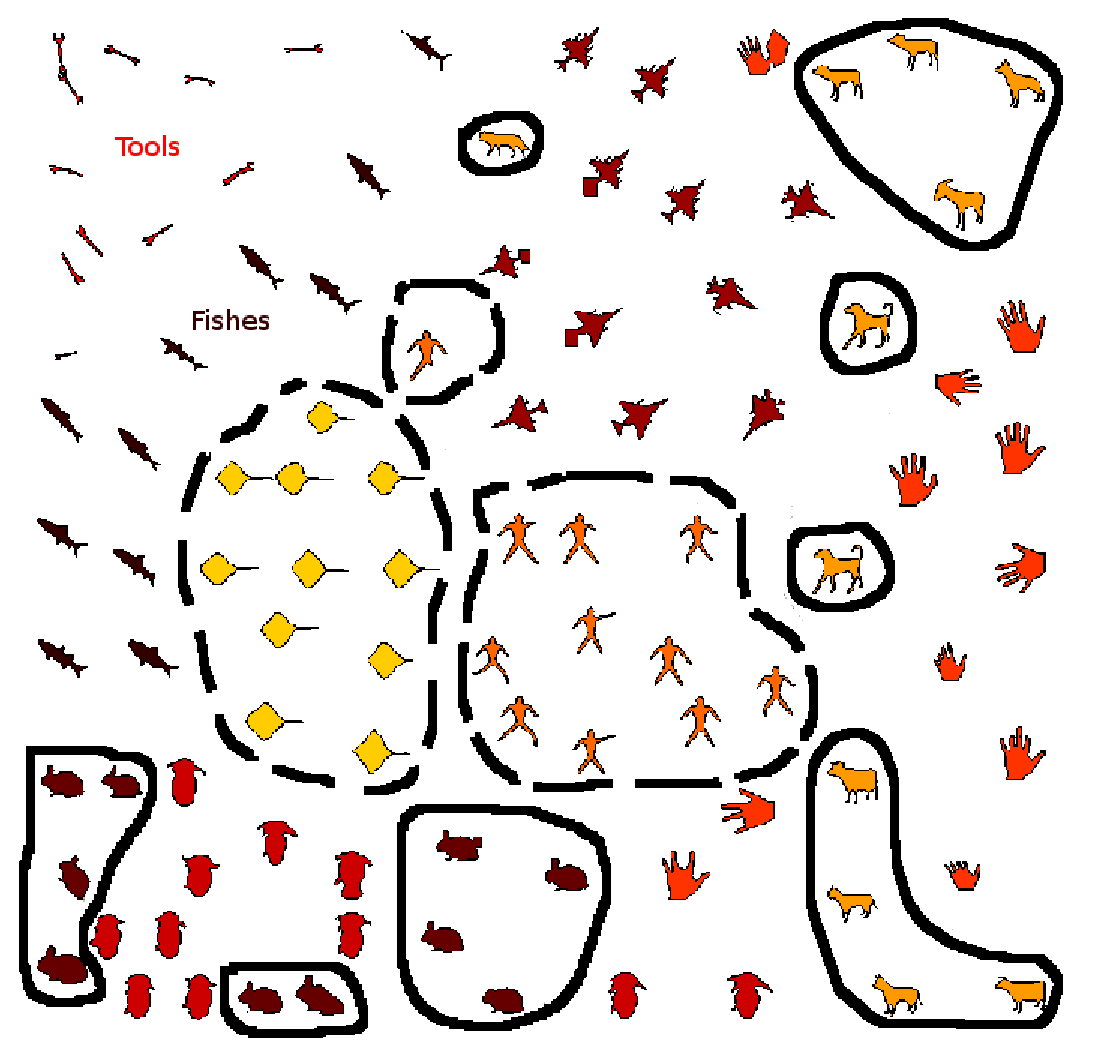
\includegraphics[width=0.5\textwidth]{nmbe_som_map_v4.eps}
\end{figure}

\begin{figure}[h!]
  \caption{\label{fig:mfd_som_map} Matriz-U para as formas da base Kimia99 representadas com o descritor Dimensão fractal multiescala.}
  \centering
  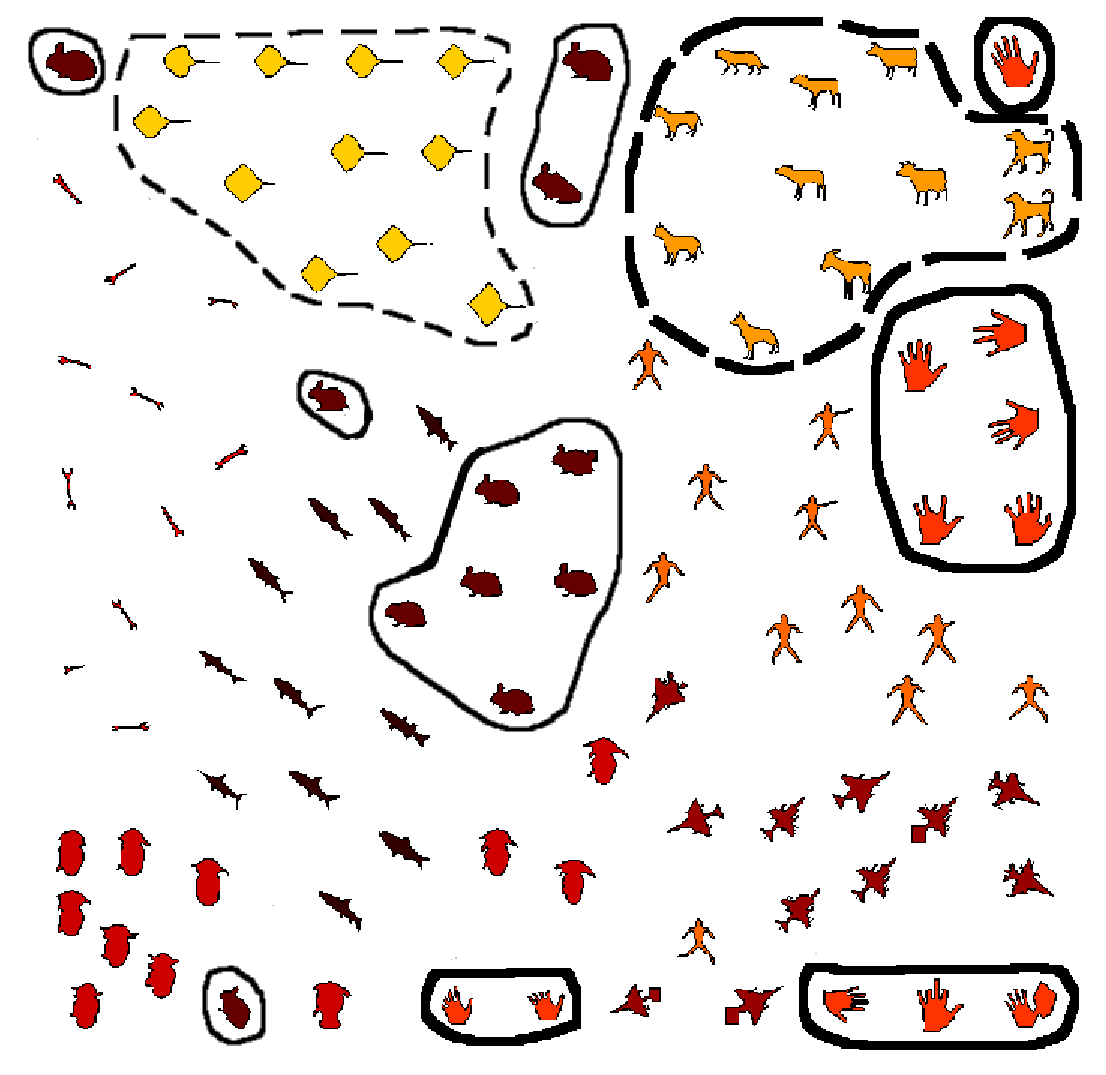
\includegraphics[width=0.5\textwidth]{mfd_som_map_v3.eps}
\end{figure}
  
\begin{figure}[h!]  \caption{\label{fig:som_kimia_216} Para o descritor energia de dobramento multiescala e a base Kimia-216: (a) Matriz-U. (b) Alguns resultados de recuperação de formas pelo conteúdo.}
  \centering
  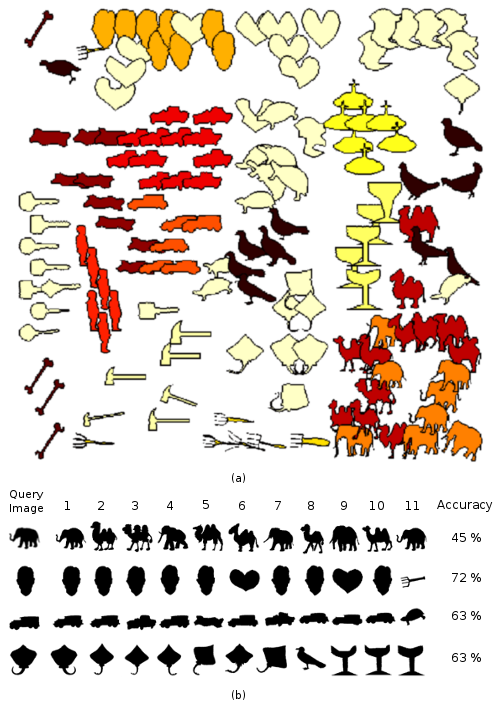
\includegraphics[width=0.5\textwidth]{retr_som_kimia216_v2.png}
\end{figure}

Já a Figura \ref{fig:som_kimia_216}a apresenta os resultados da visualização das formas da base Kimia-216 representadas através do descritor \emph{NMBE}. No canto inferior direito desta figura observamos que o descritor confunde formas dos elefantes com as dos camelos. Essa confusão aparece também no experimento de recuperação de formas pelo conteúdo (Figura \ref{fig:som_kimia_216}b), em que uma dentre as formas dos elefantes é utilizada como protótipo para se recuperar as onze formas mais similares ao protótipo na referida base.

Analogamente, no canto superior esquerdo da Figura \ref{fig:som_kimia_216}a, há confusão entre os agrupamentos das formas das faces e dos corações, bem como a presença duma forma de garfo. Na segunda linha da Figura \ref{fig:som_kimia_216}b observamos a presença dessas formas indesejáveis no experimento de recuperação de formas quando uma forma de face é apresentada como protótipo. 

Os demais resultados de recuperação de formas, apresentados na Figura \ref{fig:som_kimia_216}b, também estão coerentes com as observações da matriz-U. Nessa última podemos observar que o grupo das formas das arraias são mapeadas vizinhas aos grupos das formas dos cálices e dos pássaros, o que resulta no aparecimento das formas dessas últimas classes quando se realiza a recuperação de arraias. 

Outro aspecto importante de ser observado é que  grupos de formas com similaridades grosseiras encontram-se mapeados próximos uns dos outros na matriz-U. Formas alongadas, por exemplo, estão organizadas na parte inferior esquerda da Figura \ref{fig:som_kimia_216}a, enquanto formas arredondadas encontram-se na parte superior. Outros exemplos incluem os seguintes grupos: chaves e crianças (esquerda da figura), carros e tijolos, tartarugas e pássaros, cálices e sepulturas. 

\begin{figure}[h!]
  \caption{\label{fig:silhouette} Silhouette média por classe aferida, com a base Kimia-99, para os descritores (a) Dimensão fractal multiescala; (b) Energia de dobramento multiescala.}
  \centering
  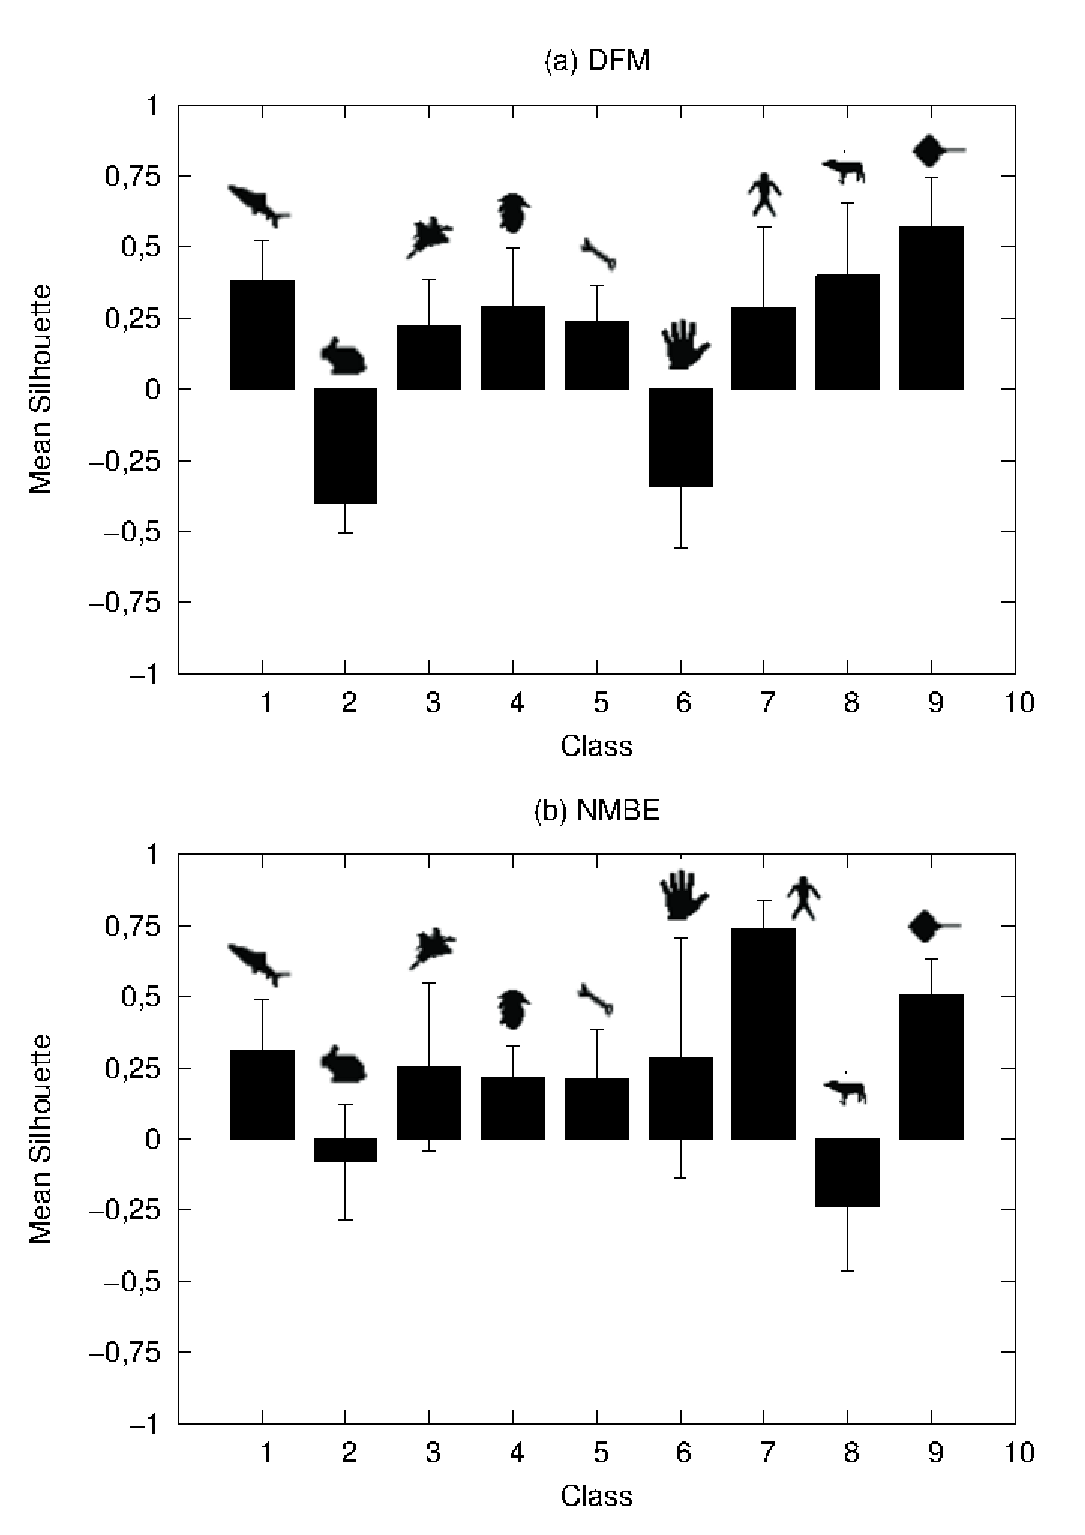
\includegraphics[width=0.5\textwidth]{resultado_silhouette.eps}
\end{figure}

\begin{figure}[h!]
  \caption{\label{fig:dude_tool_mfd}   Vetores de características calculados para amostras das formas de humanos e de ferramentas com o descritor dimensão fractal multiescala.}
  \centering
  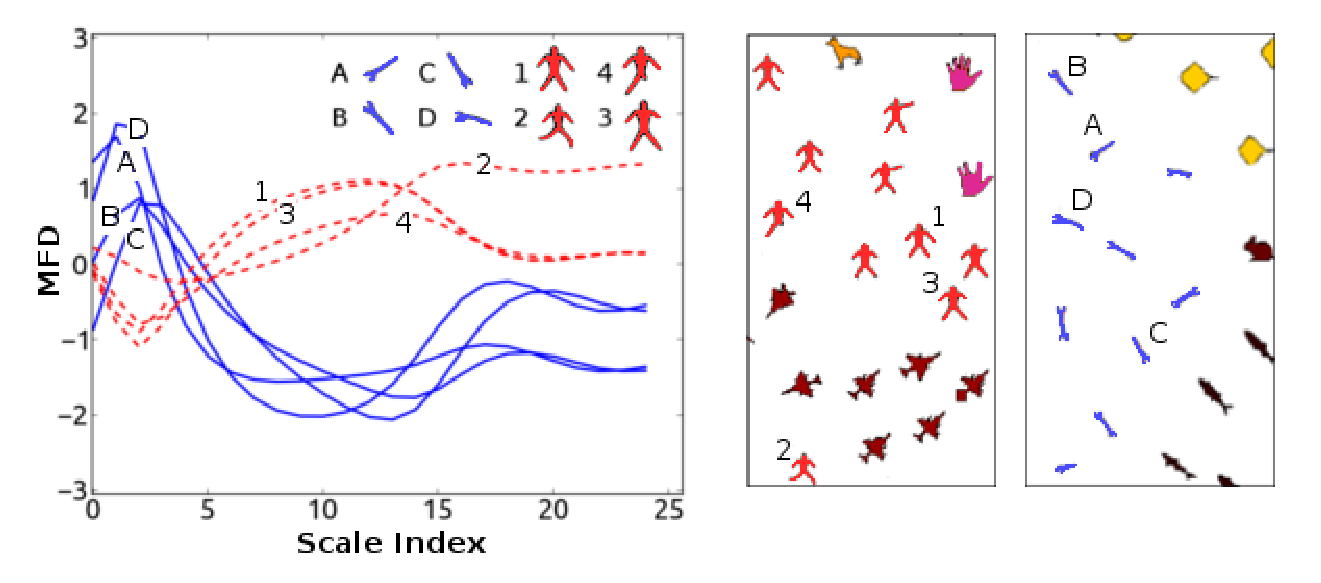
\includegraphics[width=0.75\textwidth]{dude_tool_mfd_v6.eps}
\end{figure}

\begin{figure}[h!]
  \caption{\label{fig:dude_tool_nmbe} Vetores de características calculados para amostras das formas de humanos e de ferramentes com o descritor energia de dobramento multiescala.}
  \centering
  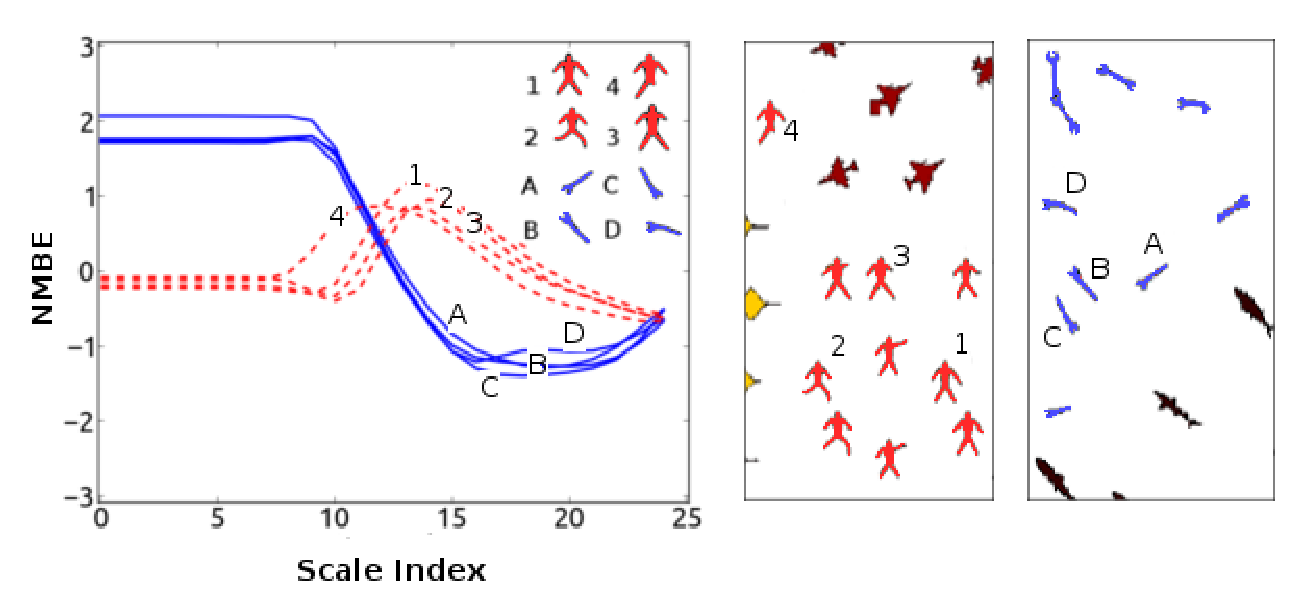
\includegraphics[width=0.75\textwidth]{dude_tool_nmbe_v6.eps}
\end{figure}

\subsection{Entropia diferencial da curvatura multiescala}

A visualização de dados obtida para características extraídas com o descritor entropia diferencial da curvatura multiescala, para a base Kimia-99, está apresentada na Figura \ref{fig:edif99}a. Nesta figura observamos a Matriz-U, em tons de cinza, sobreposta às figuras das formas nas posições mapeadas pela rede SOM.

As células escuras formam contornos que delimitam fronteiras existentes entre agrupamentos de formas, pois estas células indicam a existência duma relação de separação entre as formas em suas vizinhanças. Já as células em linhas claras indicam maior proximidade entre as formas e suas vizinhanças.

Podemos inferir que o descritor representou adequadamente as formas das classes de humanos, arraias, peixes, ferramentas e coelhos. Isso porque, nestes casos, o descritor apresentou uma representação compacta, agrupando próximas as formas de uma mesma classe, e propiciando separabilidade entre os agrupamentos estabelecidos. A medida Silhouette média por classe, apresentada na Figura \ref{fig:edif99}b, corrobora nossas observações, pois as referidas classes são as que apresentam os valores de Silhouette média mais positivos e com pequeno desvio padrão.  

Por outro lado, o descritor falhou em representar as formas das classes de animais quadrúpedes, aviões e extra terrestres. Isso porque, nesses casos, não se consegue identificar na matriz-U fronteiras claras que estabeleçam um único agrupamento das formas de uma mesma classe. Em outras palavras, formas dessas classes encontram-se separadas umas das outras ou dispersas em sub-grupos delimitados por pequenas fronteiras. Esses casos são os que apresentam a medida Silhouette média por classe com os menores valores e os maiores desvios padrão. 

Já na Figura \ref{fig:edif216}a temos a visualização da matriz-U para as características extraídas das formas da base Kimia-216. Nesta observamos, bem delimitados por linhas escuras, diversos agrupamentos  representados corretamente pelo descritor. Dentre esses, destacamos os agrupamentos cujas fronteiras de separação intra-classe são de baixo contraste e cujas fronteiras de separação inter-classe são bem contrastadas (faces, garfos, sepulturas, cálices e crianças). Esses são os  agrupamentos que apresentaram os maiores valores de \emph{Silhouette} média na Figura \ref{fig:edif216}b, o que é um resultado esperado, uma vez que o descritor representou as formas desses grupos de forma compacta e em agrupamentos bem separados.

\begin{figure}
\caption{\label{fig:edif_som_map} Matriz-U para as formas da base Kimia99 representadas com o descritor Entropia diferencial da curvatura multiescala.}
  \centering
  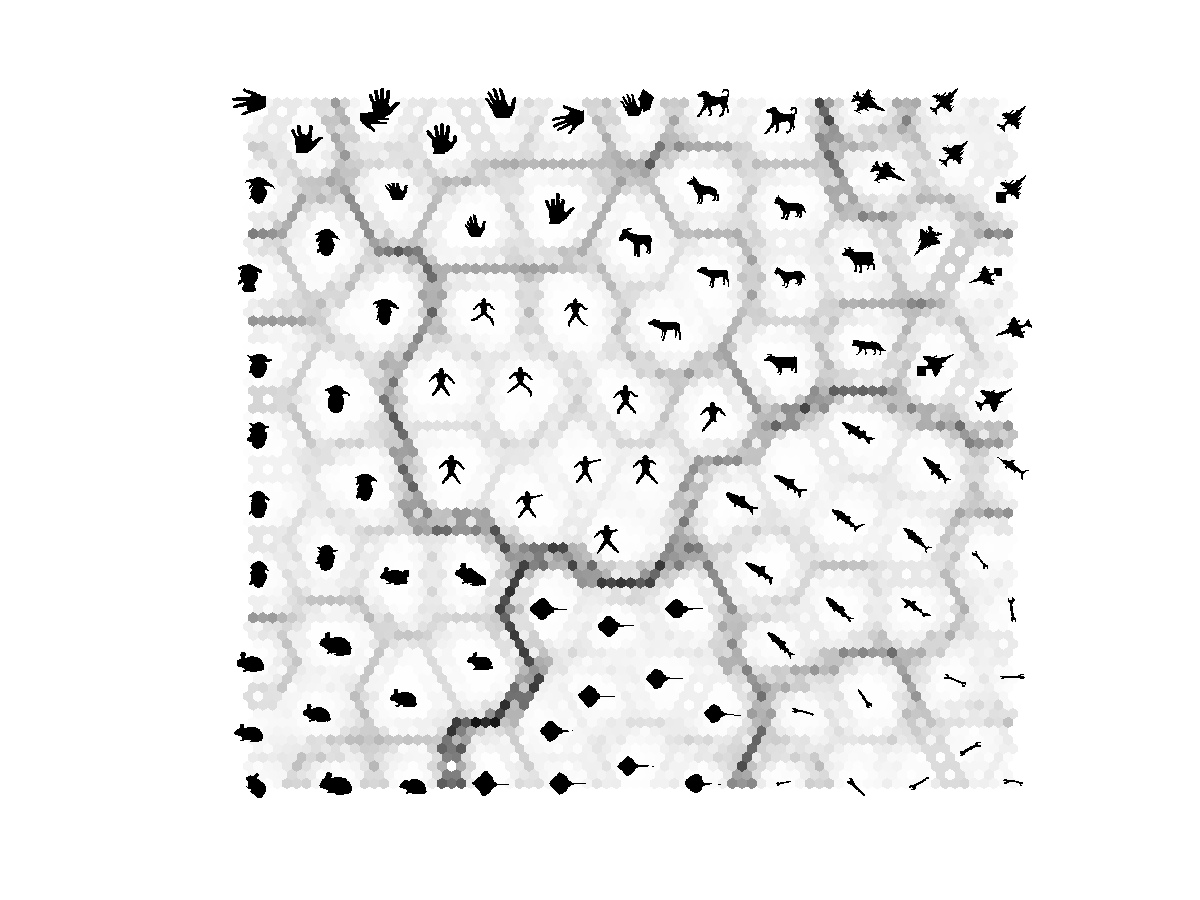
\includegraphics[width=\textwidth]{ediferencial_N5_formas.png}
 \end{figure}

\begin{figure}
\caption{\label{fig:silhouette_ediferencial} Silhouette média por classe aferida, com a base Kimia-99, para o descritor entropia diferencial da curvatura multiescala.}
  \centering
  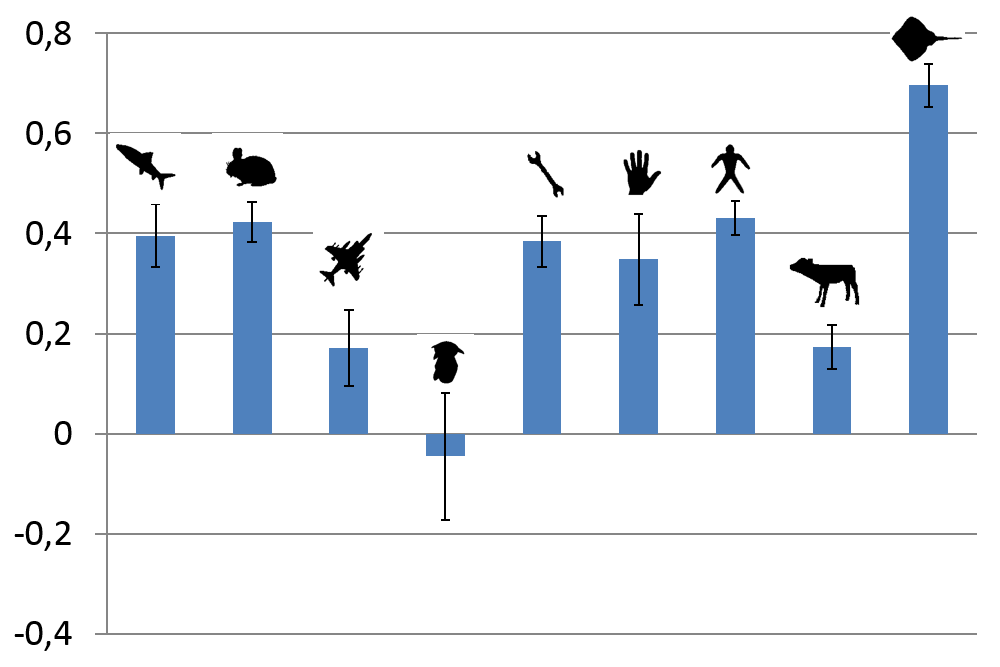
\includegraphics[width=0.75\textwidth]{ediferencial_silhouette_N5.png}
\end{figure}

\begin{figure}[h!]
  \caption{\label{fig:som_nmbe} Visualização dos dados obtida com o mapa auto-organizável de Kohonen para a descrição \emph{NMBE}.}
  \centering
  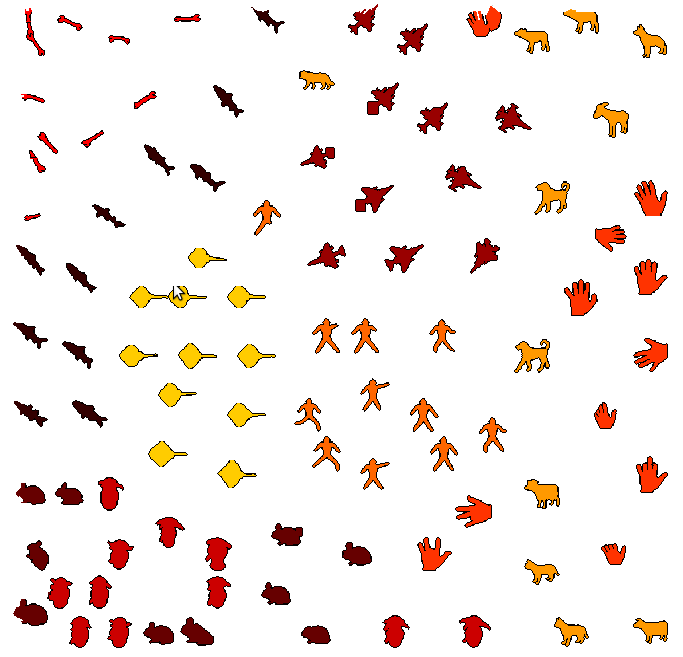
\includegraphics[width=0.5\textwidth]{mapa_som_descritor_nmbe.png}
\end{figure}

\begin{figure}[h!]
  \caption{\label{fig:som_dfm} Visualização dos dados obtida com o mapa auto-organizável de Kohonen para a descrição \emph{NMBE}.}
  \centering
  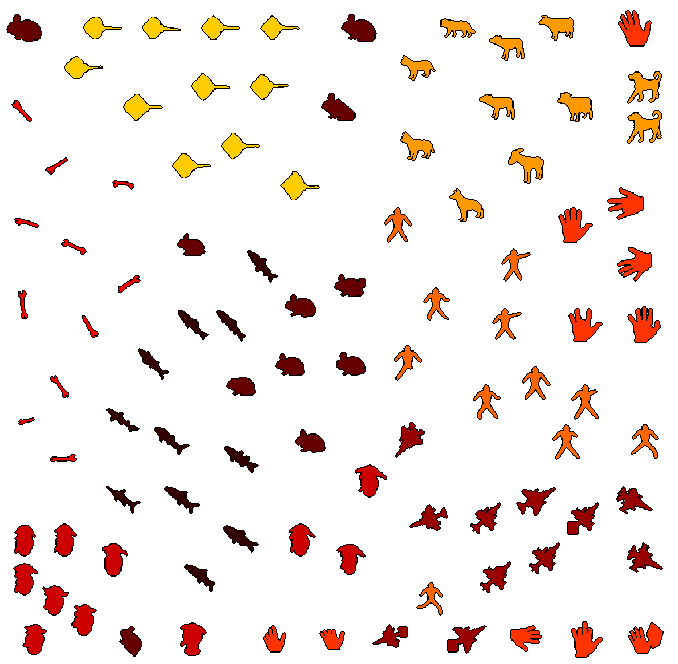
\includegraphics[width=0.5\textwidth]{mapa_som_descritor_dfm.png}
\end{figure}

\section{Recuperação de imagens pelo conteúdo}

\begin{table*}
\centering
\caption{\label{tab:KimiaChernoff} Total de acertos por classe e por posição, nos experimentos \emph{CBIR}, com a distância de Chernoff.}
\begin{tabular}{l| r r r r r r r r r r r}
\hline
&\multicolumn{11}{l}{nth nearest match} \\
\cline{2-12}
Classe&1&2&3&4&5&6&7&8&9&10&11 \\
 \hline
Peixes&11&11&11&11&9&5&8&3&7&5&5\\
Coelhos&11&11&11&11&11&11&11&11&11&11&7\\ 
Aviões&11&10&8&8&7&7&7&5&2&1&1\\
ETs&11&11&11&11&11&11&11&11&8&7&5\\
Ferramentas&11&8&7&10&3&9&9&5&7&9&9\\
Mãos&11&11&11&11&11&11&11&11&11&9&7\\
humanos&11&11&11&11&11&11&11&11&11&11&11\\
Quadrupedes&11&11&9&8&8&7&8&3&5&8&4\\
Arraias&11&11&11&11&11&11&11&10&11&9&7\\
\hline
Total&99&95&90&92&82&83&87&70&73&70&56\\
\hline
\end{tabular}
\end{table*}

\begin{table*}
\centering
\caption{\label{tab:KimiaChi-square} Total de acertos por classe e por posição, nos experimentos \emph{CBIR}, com a distância de Chi-square.}
\begin{tabular}{l| r r r r r r r r r r r}
\hline
&\multicolumn{11}{l}{nth nearest match} \\
\cline{2-12}
Classe&1&2&3&4&5&6&7&8&9&10&11 \\
 \hline
Peixes&11&11&11&10&10&8&7&9&4&4&3\\
Coelhos&11&10&10&10&10&10&10&10&10&8&1\\ 
Aviões&11&11&11&9&9&9&8&5&2&2&2\\
ETs&11&11&11&10&11&10&11&10&10&8&7\\
Ferramentas&11&11&11&11&11&11&11&11&10&11& 11\\
Mãos&11&11&11&11&11&11&11&11&11&11&9\\
humanos&11&11&11&11&11&11&11&11&11&11&11\\
Quadrupedes&11&11&6&9&8&7&7&5&7&7&4\\
Arraias&11&11&11&11&11&11&11&10&11&11&10\\
\hline
Total&99&98&93&92&92&88&87&82&76&73&58\\
\hline
\end{tabular}
\end{table*}

\begin{table*}
\centering
\caption{\label{tab:KimiaHellinger} Total de acertos por classe e por posição, nos experimentos \emph{CBIR}, com a distância de Hellinger.}
\begin{tabular}{l| r r r r r r r r r r r}
\hline
&\multicolumn{11}{l}{nth nearest match} \\
\cline{2-12}
Classe&1&2&3&4&5&6&7&8&9&10&11 \\
 \hline
Peixes&11&11&11&10&10&9&5&8&8&2&2\\
Coelhos&11&11&11&11&11&10&10&10&11&8&2\\ 
Aviões&11&11&11&10&9&11&9&8&1&1&0\\
ETs&11&11&11&11&10&11&10&11&11&7&4\\
Ferramentas&11&11&11&11&11&11&11&10&11&11& 10\\
Mãos&11&11&11&11&11&11&11&11&11&11&8\\
humanos&11&11&11&11&11&11&11&11&11&11&11\\
Quadrupedes&11&11&7&9&6&6&5&7&9&5&4\\
Arraias&11&11&11&11&11&11&11&11&11&10&9\\
\hline
Total&99&99&95&95&90&91&83&87&84&66&50\\
\hline
\end{tabular}
\end{table*}

\begin{table*}
\centering
\caption{\label{tab:KimiaJensen-Shannon} Total de acertos por classe e por posição, nos experimentos \emph{CBIR}, com a distância Jensen-Shannon.}
\begin{tabular}{l| r r r r r r r r r r r}
\hline
&\multicolumn{11}{l}{nth nearest match} \\
\cline{2-12}
Classe&1&2&3&4&5&6&7&8&9&10&11 \\
 \hline
Peixes&11&11&11&10&10&8&7&7&7&4&1\\
Coelhos&11&10&10&10&10&10&10&10&9&8&2\\ 
Aviões&11&11&10&10&9&8&8&6&3&1&1\\
ETs&11&11&11&10&11&10&10&11&9&8&5\\
Ferramentas&11&11&11&11&11&11&11&11&10&11& 11\\
Mãos&11&11&11&11&11&11&11&11&11&11&9\\
humanos&11&11&11&11&11&11&11&11&11&11&11\\
Quadrupedes&11&11&7&8&8&5&3&8&8&7&4\\
Arraias&11&11&11&11&11&11&11&11&10&11&10\\
\hline
Total&99&98&93&92&92&85&82&86&78&72&54\\
\hline
\end{tabular}
\end{table*}

\begin{table*}
\centering
\caption{\label{tab:KimiaPatrick-Fisher} Total de acertos por classe e por posição, nos experimentos \emph{CBIR}, com a distância Patrick-Fisher.}
\begin{tabular}{l| r r r r r r r r r r r}
\hline
&\multicolumn{11}{l}{nth nearest match} \\
\cline{2-12}
Classe&1&2&3&4&5&6&7&8&9&10&11 \\
 \hline
Peixes&11&11&11&10&10&9&8&5&4&1&1\\
Coelhos&11&9&9&9&9&10&10&9&7&4&4\\ 
Aviões&11&11&10&9&8&9&7&5&3&2&2\\
ETs&11&11&11&10&9&9&9&9&7&6&5\\
Ferramentas&11&10&11&11&11&10&11&11&7&9  &7\\
Mãos&11&11&11&11&11&11&11&11&11&11&9\\
humanos&11&11&11&11&11&11&11&11&11&11&10\\
Quadrupedes&11&11&8&9&8&7&5&5&7&6&6\\
Arraias&11&11&11&11&11&11&10&10&11&9&6\\
\hline
Total&99&96&93&91&88&87&82&76&68&59&50\\
\hline
\end{tabular}
\end{table*}


\begin{figure}[h!]
  \caption{\label{fig:graph1} Gráficos precisão/revocação para diferentes combinações de assinaturas. Resultados obtidos nos experimentos de recuperação de formas pelo conteúdo, com a base de imagens MPEG-7, empregando como medida de similaridade o divergente de Hellinger. }
  \centering
  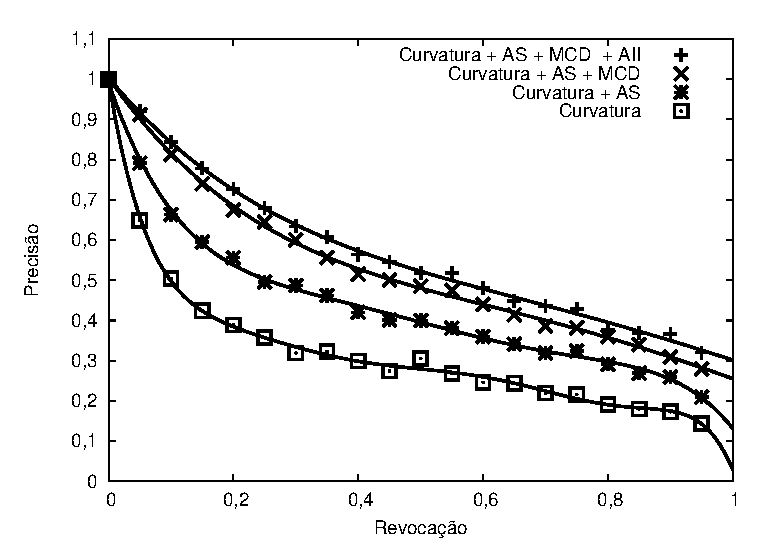
\includegraphics[width=0.75\textwidth]{graph1.eps}
\end{figure}


\section{\emph{Gap semântico}}
Uma questão importante nos sistemas \emph{CBIR} é que, embora os usuários busquem por imagens similares do ponto de vista semântico, o sistema provê os resultados com base na similaridade da informação extraída do conteúdo visual das imagens. A disparidade existente entre esses aspectos (semântica e conteúdo visual) é denominado de \emph{Gap} semântico.

Embora as imagens transmitam determinadas mensagens ao usuário, muito frequentemente os atributos extraídos das mesmas não conseguem representar e caracterizar essas mensagens. Diversos métodos para associar informação semântica aos atributos extraídos das imagens têm sido foco de pesquisa, como por exemplo solicitar que o usuário retro-alimente o sistema com o grau de relevância dos resultados obtidos (relevance feedback). 

\section{Base de imagens}

Um aspecto importante em \emph{CBIR} está ligado ao mecanismo de indexação empregado no acesso a informação contida na base de imagens. Em aplicações práticas, que requerem acesso a uma extensa base de dados, e aonde há interação dos usuários com o mecanismo de busca, o desempenho computacional no processo de indexação não pode ser negligenciado. Desta forma, armazenar vetores de características em um arquivo linear, com um registro para cada vetor, resulta na indexação sequencial destes elementos tornando essa abordagem inviável.

Todavia, mecanismos alternativos de indexação tradicionalmente encontrados na literatura, tais como \emph{k-d-b tree}, \emph{quad-tree} e \emph{R-tree} são considerados inadequados em \emph{CBIR} porque o desempenho destes se degrada substancialmente com o aumento da dimensionalidade dos dados. Ademais, para alcançar a eficiência computacional requerida sem degradar a qualidade das buscas, tais mecanismos devem levar em consideração a representação das características das imagens no processo de recuperação, ou seja, não só apenas \emph{como} indexar elementos na base de dados, mas também \emph{o que} indexar.

\end{comment}
